\documentclass{AeroStructure-ERJohnson}
\input crosslink.tex

%\usepackage{showframe}
\def\ShowFrameLinethickness{0.125pt}

\def\harp#1{\smash{\mathord{\buildrel{\lower3pt\hbox{$\scriptscriptstyle\rightharpoonup$}}\over{#1}}}}

\myexternaldocument{App_4P}
\myexternaldocument{Ch01_4P}
\myexternaldocument{Ch02_4P}
\myexternaldocument{Ch03_4P}
\myexternaldocument{Ch04_4P}
\myexternaldocument{Ch05_4P}
\myexternaldocument{Ch06_4P}
\myexternaldocument{Ch07_4P}
\myexternaldocument{Ch08_4P}
\myexternaldocument{Ch09_4P}
\myexternaldocument{Ch10_4P}
%\myexternaldocument{Ch11_4P}
\myexternaldocument{Ch12_4P}
\myexternaldocument{Ch13_4P}
\myexternaldocument{Ch14_4P}
\myexternaldocument{Ch15_4P}
\myexternaldocument{Ch16_4P}
\myexternaldocument{Ch17_4P}
\myexternaldocument{Ch18_4P}


\begin{document}


\mainmatter

\setcounter{page}{289}
\setcounter{chapter}{10}

\chapter[Buckling of columns and plates]{Buckling of columns\break and plates} \label{ch11}

If buckling occurs before the elastic limit of the material, which is roughly the yield strength of the material, then it is called \textit{elastic buckling}. If buckling occurs beyond the elastic limit, it is called \textit{inelastic buckling}, or plastic buckling if the material exhibits plasticity during buckling (mainly metals). Many thin-walled structural components buckle in compression below the elastic limit. Therefore, buckling determines the limit state in compression rather than material yielding. In fact, about 50 percent of an airplane structure is designed based on buckling\break constraints.

\vspace*{-1pc}

\section{Perfect columns}\label{sec11.1}



Consider\enlargethispage{-1\baselineskip} a perfectly straight, uniform column of length \textit{L} with cross-sectional area \textit{A} subject to a centric end load \textit{P} as shown in figure~\ref{fig11.1}. (The column is drawn horizontally for convenience.) The column is long relative to its largest cross-sectional dimension, and the column consists of a homogeneous, linear elastic material whose modulus of elasticity is denoted by \textit{E}. Buckling analyses are inherently nonlinear. As the previous structural models discussed in chapter 10 demonstrate, nonlinear analysis results in more than one equilibrium state for a specified load, whereas in linear analysis there is only one equilibrium state for a specified load. A geometrically nonlinear analysis of a column is developed in this article in which the axial strain-displacement relation is nonlinear and equilibrium is taken on the displaced structure.


\begin{figure}[!h]
\centerline{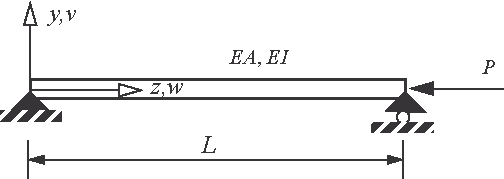
\includegraphics{Figure_11-1.pdf}}
\caption{A straight column subject to a centric, compressive axial force.} \label{fig11.1}
\end{figure}

\subsubsection{Kinematics.} Consider a differential element \textit{dz}-by-\textit{dy} in the initial, undeformed column, where \textit{dz} is along the centroidal axis and \textit{dy} is perpendicular to the centroidal axis as shown in figure~\ref{fig11.2}. In the \textit{z-y} coordinate system, the material point at coordinates (\textit{z, 0}) displaces to coordinates (\textit{z*, y*}) in the deformed bar, where\break (\textit{z*, y*}) is referenced to the same \textit{z-y} system. These coordinates are related by
\begin{align}\label{eq11.1}
 z^{*}=z+w(z) \quad y^{*}=0+v(z) ,
\end{align}
where $w(z)$ is the displacement parallel to the $z$-axis and $ v(z) $ is the displacement parallel to the $y$-axis. The material points along length \textit{dz} map to the differential length \textit{ds*} along the centroidal axis in the deformed bar. By the Pythagorean theorem $ \left(d s^{*}\right)^{2}=\left(d z^{*}\right)^{2}+\left(d y^{*}\right)^{2} $. The differential lengths in the deformed bar are
\begin{equation}
d z^{*}=\left(1+\frac{d w}{d z}\right) d z\,\textrm{and } d y^{*}=\left(\frac{d v}{d z}\right) d z. \label{eq11.2}
\end{equation}
Define the stretch ratio $\lambda$ by $\lambda=d s^{*}/dz$. Consequently, the stretch ratio is related to the derivatives of the displacements by
\begin{figure}[!h]
\centerline{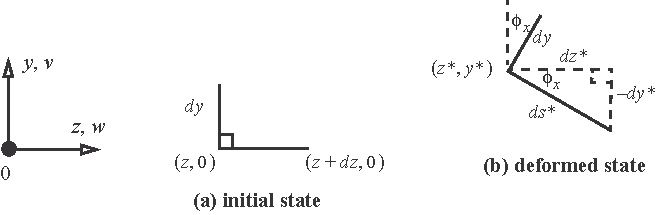
\includegraphics{Figure_11-2.pdf}}
\caption{Differential elements in the initial state (a) and in the deformed state (b).} \label{fig11.2}
\end{figure}
\begin{align}\label{eq11.3}
 \lambda=\sqrt{\left(1+\frac{d w}{d z}\right)^{2}+\left(\frac{d v}{d z}\right)^{2}}.
\end{align}
The clockwise rotation angle of element \textit{ds}* with respect to the $z$-direction is denoted by $ \phi_{x}(z) $. Trigonometric functions of this rotation angle are given by
\begin{align}\label{eq11.4}
 \sin \phi_{x}=\frac{-d y^{*}}{d s^{*}}\,\textrm{and } \cos\phi_{x}=\frac{d z^{*}}{d s^{*}}.
\end{align}
\noindent Using the chain rule of differentiation and the definition of the stretch ratio these trigonometric functions can be written as
\begin{align}\label{eq11.5}
 \sin \phi_{x}=\left(\frac{-d y^{*}}{d z}\right) \frac{d z}{d s^{*}}=\frac{1}{\lambda}\left(\frac{-d v}{d z}\right),\,\textrm{ and similarly } \cos\phi_{x}=\frac{1}{\lambda}\left(1+\frac{d w}{d z}\right).
\end{align}
We impose the hypothesis of classical theory that cross sections normal to the centroidal axis in the undeformed bar remain rigid and normal to the centroidal axis in the deformed bar. Thus, the differential line element \textit{dy} in the undeformed bar does not change length in the deformed bar and remains normal to the centroidal\vadjust{\vspace*{8pt}\pagebreak} axis in the deformed bar. That is, line element \textit{dy} also rotates clockwise through angle $ \phi_{x}$. The stretch ratio (\ref{eq11.3}) is expanded in a binomial series to\vspace*{-3pt} get
\begin{equation}
\lambda=1+\frac{1}{2}\left[2 \frac{d w}{d z}+\left(\frac{d w}{d z}\right)^{2}+\left(\frac{d v}{d z}\right)^{2}\right]-\frac{1}{8}\left[2 \frac{d w}{d z}+\left(\frac{d w}{d z}\right)^{2}+\left(\frac{d v}{d z}\right)^{2}\right]^{2}+\ldots=1+\frac{d w}{d z}+\frac{1}{2}\left(\frac{d v}{d z}\right)^{2}+O\left(\frac{d w}{d z}\right)^{3}. \label{eq11.6}
\end{equation}
The engineering strain is defined as $\varepsilon_{z z}=\lambda-1$. If cubic powers and higher of the displacement derivatives in the series expansion of $ \lambda $ are neglected, then the strain-displacement relation\vspace*{-3pt} is
\begin{equation}
\varepsilon_{z z}=\frac{d w}{d z}+\frac{1}{2}\left(\frac{d v}{d z}\right)^{2}. \label{eq11.7}
\end{equation}



\subsubsection{Equilibrium.} The free body diagram of the element of the bar in the deformed state is shown in figure~\ref{fig11.3}(a). The force \textit{F} acting on the cross section of the deformed bar is resolved in two sets of orthogonal components. Components \textit{H} and $S_{y}$ act in horizontal direction and the vertical direction, respectively. Components \textit{N} and $V_{y}$ act tangent and normal to the centroidal axis, respectively. Let $\alpha$ denote the angle between the vertical and the line of action of force \textit{F}. From figure~\ref{fig11.3}(b) $H=F\sin\alpha$ and $S_{y}=F \cos \alpha$. Components \textit{N} and $V_{y}$ are given\vspace*{-5pt} by
\begin{figure}[!h]
\centerline{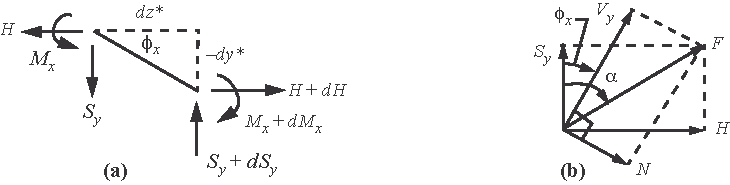
\includegraphics{Figure_11-3.pdf}}
\caption{Free body diagram of the differential element in the deformed bar (a), and the resolution of the resultant force $F$ into components acting on the cross section (b).} \label{fig11.3}\vspace*{-5pt}
\end{figure}
\begin{gather}
N=F \sin \left(\alpha-\phi_{x}\right)=(F \sin \alpha) \cos \phi_{x}-(F \cos \alpha) \sin \phi_{x}=H \cos \phi_{x}-S_{y} \sin \phi_{x} ,\,\textrm{and} \label{eq11.8}\\
V_{y}=F \cos \left(\alpha-\phi_{x}\right)=(F \cos \alpha) \cos \phi_{x}+(F \sin \alpha) \sin \phi_{x}=S_{y} \cos \phi_{x}+H \sin \phi_{x}. \label{eq11.9}
\end{gather}
Equilibrium in the horizontal direction requires $dH=0$ and equilibrium in the vertical direction requires $ d S_{y}=0 $. Thus, the horizontal component \textit{H} and the vertical component $ S_{y} $ are spatially uniform along the length of the bar. Since the applied compressive force \textit{P} is also horizontal then $ H=-P $. The bending moment is denoted by $M_{x}$. Moment equilibrium about the right end of the element in figure~\ref{fig11.3}(a) leads to
\begin{align}\label{eq11.10}
 M_{x}+d M_{x}-M_{x}-\left(-d y^{*}\right) H-\left(d z^{*}\right) S_{y}=0.
\end{align}
The differential functions are expanded in a series. For example $ d M_{x}=\frac{d M_{x}}{d z} d z+\frac{d^{2} M_{z}}{d z^{2}}\left(d z^{2}\right)+\ldots.$ Then moment equilibrium becomes
\begin{align}\label{eq11.11}
 \left[\frac{d M_{x}}{d z}-\left(\frac{-d y^{*}}{d z}\right) H-\left(\frac{d z^{*}}{d z}\right) S_{y}\right] d z+O\left(d z^{2}\right)=0.
\end{align}
Division by \textit{dz} followed by the limit as $ d z \rightarrow 0 $ leads to the differential equation
\begin{equation}
\frac{d M_{x}}{d z}-\left(\frac{d v}{d z}\right) p-\left(1+\frac{d w}{d z}\right) S_{y}=0. \label{eq11.12}
\end{equation}
\vspace*{5pt}
\clearpage

\subsubsection{Hooke's law.} The normal force component \textit{N} is proportional to the axial strain $\varepsilon_{zz}$ of the centroidal axis, and the bending moment $M_{x}$ is proportional to the rotation gradient $\frac{d \phi_{x}}{d z}$ of the cross section. That is,
\begin{equation}
N=\textit{E A} \varepsilon_{z z} \quad M_{x}=E I\left(\frac{d \phi_{x}}{d z}\right), \label{eq11.13}
\end{equation}
where the modulus of elasticity is denoted by \textit{E}, the cross-sectional area by \textit{A}, and the second area moment of the cross section by \textit{I}.

\subsection{Pre-buckling equilibrium}\label{sec11.1.1}

The trivial equilibrium configuration of the column is straight and in compression subject to the applied axial force \textit{P}. The lateral displacement $ v(z)=0 $, rotation $ \phi_{x}(z)=0 $, and $ M_{x}=0 $ for $ 0 \leq z \leq L $. From eq.~(\ref{eq11.8}) ${N=H=-P}$. From eq.~(\ref{eq11.9}) $ S_{y}=V_{y} $ but overall equilibrium requires $ S_{y}=0 $. Let $ w_{0}(z) $ denote the axial displacement in pre-buckling equilibrium. Then, strain (\ref{eq11.7}) and stretch ratio reduce to $\varepsilon_{zz}=\frac{d w_{0}}{d z} $ and $ \lambda=1+\frac{d w_{0}}{d z} $, respectively. Hooke's law (\ref{eq11.13}) for the axial force is $ -P=E A\left(\frac{d w_{0}}{d z}\right) $. Integrate Hooke's law and take the axial displacement $ w_{0}(0)=0 $ to get
\begin{equation}
w_{0}(z)=\frac{-P z}{E A}. \label{eq11.14}
\end{equation}

\subsection{Buckling}\label{sec11.1.2}

To assess buckling of a slightly defected column, we introduce a small, dimensionless parameter $ \xi $ such that all dependent variables equal there pre-buckling equilibrium expressions as $ \xi \rightarrow 0 $. The displacements and rotation are expressed as
\begin{equation}
w(z)=w_{0}(z)+\xi w_{1}(z) \quad v(z)=\xi v_{1}(z) \quad \phi_{x}(z)=\xi \phi_{1}(z). \label{eq11.15}
\end{equation}
The trigonometric functions of the rotation angle are
\begin{align}
\sin \phi_{x}=\xi \phi_{1}(z)+O\big(\xi^{3}\big) \quad \cos \phi_{x}=1+O\big(\xi^{2}\big).\label{eq11.16}
\end{align}
In the following developments terms of $ \xi^{2} $ and higher degrees are neglected. The vertical shear force $ S_{y}=\xi S_{y 1} $. The axial strain (\ref{eq11.7}) expansion is
\begin{equation}
\varepsilon_{zz}=\frac{d w_{0}}{d z}+\xi \frac{d w_{1}}{d z}. \label{eq11.17}
\end{equation}
The first expression in (\ref{eq11.8}) is written as $ N+P \cos \phi_{x}+S_{y} \sin \phi_{x}=0 $ , where $ N=E A \varepsilon_{z z} $. The expansion for this equation containing the force \textit{N} is
\begin{align}
\xi^{0}\left[E A \frac{d w_{0}}{d z}+P\right]+\xi\left[E A \frac{d w_{1}}{d z}\right]+O(\xi^{2})=0.\label{eq11.18}
\end{align}
To satisfy the last equation for each value of $ \xi \neq 0 $, the coefficients of $ \xi^{0} $ and $ \xi^{1} $ must vanish, which leads to
\begin{align}
\frac{d w_{0}}{d z}=\frac{-P}{E A} \quad \frac{d w_{1}}{d z}=0. \label{eq11.19}
\end{align}
On the pre-buckling equilibrium path the stretch ratio $ \lambda=1-P /(E A) $.

The expansion of the equilibrium equation for bending (\ref{eq11.12}) combined with the moment from Hooke's law (\ref{eq11.13}) is
\begin{align}
\xi^{0} \cdot 0+\xi\left[E I \frac{d^{2} \phi_{1}}{d^{2}}-P \frac{d v_{1}}{d z}-\left(1-\frac{P}{E A}\right) S_{y 1}\right]+O\big(\xi^{2}\big)=0. \label{eq11.20}
\end{align}
\vspace*{5pt}
\clearpage

\noindent Therefore, the significant result from eq.~(\ref{eq11.20}) is
\begin{align}
E I \frac{d^{2} \phi_{1}}{d z^{2}}-p \frac{d v_{1}}{d z}-\left(1-\frac{P}{E A}\right) S_{y 1}=0. \label{eq11.21}
\end{align}

\vspace*{-1pc}

The first expression in eq.~(\ref{eq11.5}) relating the rotation, the stretch ratio, and the displacement \textit{v(z)} is written as
\begin{align}
 [1-P /(E A)] \sin \phi_{x}+\frac{d v}{d z}=0. \label{eq11.22}
\end{align}
The expansion of eq.~(\ref{eq11.22}) becomes
\begin{align}
\xi^{0} \cdot 0+\xi\left[\frac{d v_{1}}{d z}+\left(1-\frac{P}{E A}\right) \phi_{1}\right]+O\big(\xi^{2}\big)=0. \label{eq11.23}
\end{align}
Therefore,
\begin{align}
\frac{d v_{1}}{d z}+\left(1-\frac{P}{E A}\right) \phi_{1}=0. \label{eq11.24}
\end{align}

\vspace*{-1pc}

Solve eq.~(\ref{eq11.24}) for $ \phi_{1}(z)$ and substitute the result into eq.~(\ref{eq11.21}) to get
\begin{align}
-E I\left[\frac{d^{3} v_{1}}{dz^{3}}\right]-P\left(1-\frac{P}{E A}\right) \frac{d v_{1}}{d z}-\left(1-\frac{P}{E A}\right)^{2} S_{y 1}=0. \label{eq11.25}
\end{align}
Now differentiate eq.~(\ref{eq11.25}) with respect to $z$ and note that $ \frac{d S_{y 1}}{d z}=0 $ consistent with the equilibrium equation $ \frac{d S_{y}}{d z}=0 $. The final result is
\begin{align}
\frac{d^{4} v_{1}}{d z^{4}}+K^{2} \frac{d^{2} v_{1}}{d z^{2}}=0 \quad v_{1}=v_{1}(z) \quad 0<z<L , \label{eq11.26}
\end{align}
where
\begin{align}
K^{2}=\frac{P}{E I}\left(1-\frac{P}{E A}\right). \label{eq11.27}
\end{align}
The expressions for the bending moment and vertical shear force are
\begin{align}
\left(1-\frac{P}{E A}\right) M_{x 1}=-E I\left(\frac{d^{2} v_{1}}{d z^{2}}\right) \quad\left(1-\frac{P}{E A}\right)^{2} S_{y 1}=-E I\left[\frac{d^{3} v_{1}}{dz^{3}}+K^{2} \frac{d v_{1}}{d z}\right]. \label{eq11.28}
\end{align}

\vspace*{-1pc}

The solution of eq.~(\ref{eq11.26}) for $ v_{1}(z) $ is subject to boundary conditions at $z= 0$ and $z =L$. There are four so-called standard boundary conditions. These are shown in figure~\ref{fig11.4}.

\begin{figure}[!t]
\vspace*{-1.6\baselineskip}
\centerline{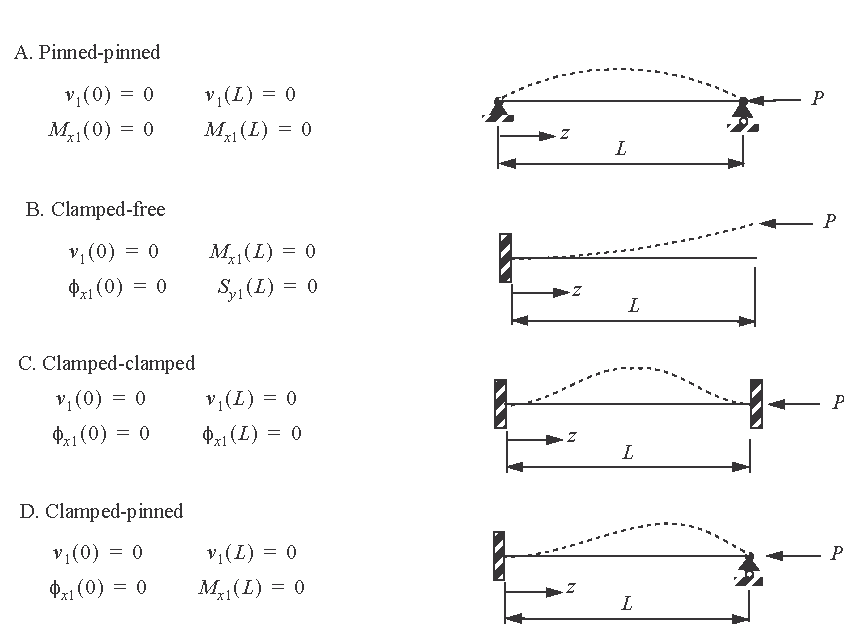
\includegraphics{Figure_11-4.pdf}}
\caption{Standard buckling boundary conditions.} \label{fig11.4}
%\vspace*{-6pt}
\end{figure}


One solution to the differential equation (\ref{eq11.26}) subject to boundary conditions A-D is $ v_{1}(z)=0 $ for all values of the load \textit{P}. This is the trivial solution. The general solution of eq.~(\ref{eq11.26}) for $ K^{2}>0 $ is
\begin{align}
v_{1}(z)=A_{1} \sin (K z)+A_{2} \cos (K z)+A_{3} z+A_{4} , \label{eq11.29}
\end{align}
where $\textit{A}_{1}$, $\textit{A}_{2}$, $\textit{A}_{3}$, and $\textit{A}_{4}$ are arbitrary constants to be determined by boundary conditions.
\vspace*{5pt}
\pagebreak

\begin{example}[Critical load for clamped-free boundary conditions in figure~\ref{fig11.4}(B)] \label{ex11.1}%
Consider the clamped-free boundary conditions denoted as (B). Determine the critical load $P_{cr}$ for which the perfect column admits a non-trivial equilibrium state.

\subsubsection{Solution.} The bending moment and vertical shear force (\ref{eq11.28}) vanish at $z = L$. The four boundary conditions in this case are
\begin{equation}
 v_{1}(0)=0 \quad v_{1}^{\prime}(0)=0 \quad E I v_{1}^{\prime \prime}(L)=0 \quad\left[v_{1}{ }^{\prime\prime\prime}+K^{2} v_{1}^{\prime}\right]_{z=L}=0 , \label{eq11.1.a}\tag{a}
\end{equation}
where the primes denote derivatives with respect to $z$. Taking derivatives of eq.~(\ref{eq11.29}) we have
\begin{gather}
v_{1}=A_{1} \sin (K z)+A_{2} \cos (K z)+A_{3} z+A_{4} \nonumber\\
v_{1}^{\prime}=A_{1} K \cos (K z)-A_{2} K \sin (K z)+A_{3} \nonumber\\
v_{1}^{\prime \prime}=-A_{1} K^{2} \sin (K z)-A_{2} K^{2} \cos (K z) \nonumber\\
v_{1}^{\prime\prime\prime}=-A_{1} K^{3} \cos (K z)+A_{2} K^{3} \sin (K z). \label{eq11.1.b}\tag{b}
\end{gather}
Substitute these solutions into the four boundary conditions to get
\begin{gather}
\left[\begin{array}{@{}cccc@{}} 0 & 1 & 0 & 1 \\ K & 0 & 1 & 0 \\ -K^{2} \sin (K L) & -K^{2} \cos (K L) & 0 & 0 \\ 0 & 0 & K^{2} & 0 \end{array}\right]\left[\begin{array}{@{}c@{}} A_{1} \\ A_{2} \\ A_{3} \\ A_{4} \end{array}\right]=0. \label{eq11.1.c}\tag{c}
\end{gather}
A non-trivial solution for $\textit{A}_1$ to $\textit{A}_4$ requires the determinate of coefficients to vanish:
\begin{equation}
\textit{det }\left[\begin{array}{@{}cccc@{}} 0 & 1 & 0 & 1 \\ K & 0 & 1 & 0 \\ -K^{2} \sin (K L) & -K^{2} \cos (K L) & 0 & 0 \\ 0 & 0 & K^{2} & 0 \end{array}\right]=0. \label{eq11.1.d}\tag{d}
\end{equation}
After expanding this determinate we get
\begin{equation}
 -K^{5} \cos (K L)=0 , \label{eq11.1.e}\tag{e}
\end{equation}
which is called the \textbf{characteristic equation}. The solution $ K=0 $ of the characteristic equation leads to the trivial solution for $ v(z) $. Non-trivial solutions to the characteristic equation occur for $\cos(KL)=0$, whose positive roots are
\begin{equation}
 K_{n} L=(2 n-1)(\pi/2) \quad n=1,2,3, \ldots. \label{eq11.1.f}\tag{f}
\end{equation}

For the discrete values of $K_{n} L$ in eq. (\textbf{\ref{eq11.1.f}}) to satisfy the equation in the fourth row of matrix eq. (\textbf{\ref{eq11.1.c}}) requires $ A_{3}=0 $. Setting $ A_{3}=0 $ in the equation in the second row of matrix eq. (\textbf{\ref{eq11.1.c}}) requires $ A_{1}=0 $. The equation of the first row of matrix eq. (\textbf{\ref{eq11.1.c}}) yields $ A_{2}=-A_{4}$. Note that the equation obtained from the third row of matrix eq. (\textbf{\ref{eq11.1.c}}) is identically satisfied for $ A_{1}=0 $ and the discrete values of $ K_{n} L $. For each value of $n$ we have an associated \textbf{buckling mode} ($A_1 = A_3 = 0$, $A_{{2}} = -A_4$):
\begin{equation}
 v_{1}(z)=A_{4}\left[1-\cos \left(K_{n} z\right)\right]. \label{eq11.1.g}\tag{g}
\end{equation}

\removelastskip

The buckling loads are determined from the expression for $K^{2}$ in eq.~(\ref{eq11.27}), which after some manipulation is written as
\begin{equation}
K^{2}=\left(\frac{P}{EI}\right)\left(1-\frac{P}{EI}\left(\frac{EI}{E A}\right)\right)=k^{2}\big(1-k^{2} r^{2}\big), \label{eq11.1.h}\tag{h}
\end{equation}
where $k^{2}=P /(E I) $ and $ r^{2}=I/A $. The radius of gyration of the cross section is denoted by $r$. At $ K=K_{1}=\pi /(2 L) $ we have
\begin{equation}
\left(\frac{\pi}{2L}\right)^{2}=k_{\mathrm{cr}}^{2}\big(1-k_{\mathrm{cr}}^{2} r^{2}\big) ,\label{eq11.1.i}\tag{i}
\end{equation}
where $k_{\mathrm{cr}}^{2}=P_{\mathrm{cr}} /(EI)$. Equation (\textbf{\ref{eq11.1.i}}) is a quadratic equation for $ k_{\mathrm{cr}}^{2} $, and the lowest root is
\begin{equation}
k_{\mathrm{cr}}^{2}=\frac{L-\sqrt{L^{2}-\pi^{2} r^{2}}}{2 L r^{2}}=\frac{1}{2 L^{2}}\left(\frac{L}{r}\right)\left[\left(\frac{L}{r}\right)-\sqrt{\left(\frac{L}{r}\right)^{2}-\pi^{2}}\;\right] , \label{eq11.1.j}\tag{j}
\end{equation}
where $L/r$ is the \textit{slenderness ratio} of the column. For selected values of the slenderness ratio the values of $ k_{\mathrm{cr}}^{2} $ are listed in table~\ref{tab11.1}.

Values of $k_{\mathrm{cr}}^{2} $ monotonically decrease with increasing slenderness ratios and approach a minimum value of $ \pi^{2} /\left(4 L^{2}\right) $ as $ L/r \rightarrow \infty $. At $ L/r=20 $ the value of $ k_{\mathrm{cr}}^{2} $ is 0.63 percent higher than the minimum, and at $ L/r=100 $ the value of $ k_{\mathrm{cr}}^{2} $ is 0.03 percent higher than the minimum. In design we use the minimum value of $ k_{\mathrm{cr}}^{2} $ for the critical load. That is,
\begin{equation}
\left[k_{\mathrm{cr}}^{2}=P_{\mathrm{cr}} /(E I)=\pi^{2} /\big(4 L^{2}\big)\right] \rightarrow P_{\mathrm{cr}}=\frac{\pi^{2} E I}{4 L^{2}}. \label{eq11.1.k}\tag{k}
\end{equation}

The result for the critical load in eq. (\textbf{\ref{eq11.1.k}}) is obtained if the axial strain at the bifurcation point with is neglected with respect to unity. From eqs. (\ref{eq11.17}) and (\ref{eq11.19}) the strain at the bifurcation point is
\begin{equation*}
\varepsilon_{z z}=\frac{d w_{0}}{d z}=-\left(\frac{P_{\textrm{cr}}}{E A}\right)=-\left(\frac{\pi^{2}}{4(I/r)^{2}}\right).
\end{equation*}
\vspace*{5pt}
\pagebreak

\begin{table}
\processtable{Buckling coefficient for selected slenderness ratios. \label{tab11.1}}{
\tabcolsep=32pt\begin{tabular}{@{}lll@{}}
\toprule
\colhead{\raisebox{-5pt}{$L/r $}} & \colhead{\raisebox{-5pt}{$k_{\textbf{cr}}^{\textbf{2}}$}} & \colhead{$\frac{k_{\textbf{cr}}^{\textbf{2}}}{\left(k_{\textbf{cr}}^{\textbf{2}}\right) \mathrm{min}} $} \\
\midrule
20 & $ 2.48281/L^{2} $ & 1.00625\\
40 & $ 2.47122/L^{2} $ & 1.00153\\
60 & $ 2.46909/L^{2} $ & 1.00069\\
80 & $ 2.46835/L^{2} $ & 1.00039\\
100 & $ 2.46801/L^{2} $ & 1.00025\\
$ \infty $ & $ \pi^{2} /\left(4 L^{2}\right)=2.4674/L^{2} $ & 1.0\\
\botrule
\end{tabular}}{}
\vspace*{-1pc}
\end{table}

\noindent For $ 20 \leq L/r \leq 100 $ the range of the strain at bifurcation point is $ -0.0062 \leq \varepsilon_{z z} \leq-0.00025 $. For small strain at the bifurcation point the stretch ratio $ \lambda=1+\varepsilon_{zz} \cong 1 $. Equation (\ref{eq11.27}) yields ${K}_{\mathrm{cr}}^{2}=k_{\mathrm{cr}}^{2} \lambda \approx k_{\mathrm{cr}}^{2}$. Hence, the values of $k$ are
\begin{equation}
k_{n}=\frac{(2 n-1)}{L} \frac{\pi}{2}=\sqrt{\frac{P_{n}}{E I}} \quad n=1,2,3, \ldots \label{eq11.1.l}\tag{l}
\end{equation}
Solve eq. (\textbf{\ref{eq11.1.l}}) for the loads to get
\begin{equation}
P_{n}=\left[(2 n-1) \frac{\pi}{2}\right]^{2} \frac{E I}{L^{2}} \quad n=1,2,3, \ldots , \label{eq11.1.m}\tag{m}
\end{equation}
where $P_{\textrm{n}}$ are the \textbf{buckling loads}. The first three buckling modes and corresponding buckling loads are shown in figure~\ref{fig11.5}. Remember that in design we use the minimum \textit{EI} for the cross section.
\end{example}

\begin{figure}[!h]
\centerline{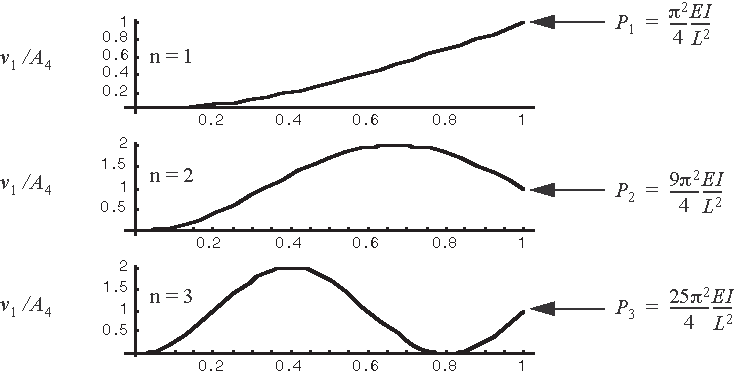
\includegraphics{Figure_11-5.pdf}}
\caption{First three buckling modes for the clamped-free column.} \label{fig11.5}
\end{figure}

\subsection{Buckling equations for negligible strain at the bifurcation point}\label{sec11.1.3}

Neglecting the axial strain with respect to unity means the stretch ratio $\lambda=1-P /(E A) \approx 1 $, and eqs. (\ref{eq11.21}), (\ref{eq11.24}), and (\ref{eq11.27}) simplify\vspace*{8pt} to\pagebreak
\begin{align}
EI \frac{d^{2} \phi_{1}}{d z^{2}}-P \frac{d v_{1}}{d z}-S_{y 1}=0 \quad \frac{d v_{1}}{d z}+\phi_{1}=0 \quad K^{2}=\frac{P}{E I} \quad 0<z<L, \label{eq11.30}
\end{align}
From eq.~(\ref{eq11.26}) the differential equation governing buckling is
\begin{align}
\frac{d^{4} v_{1}}{d z^{4}}+k^{2} \frac{d^{2} v_{1}}{d z^{2}}=0 \quad v_{1}=v_{1}(z) \quad 0<z<L \quad k^{2}=P /(E I). \label{eq11.31}
\end{align}

The critical loads for boundary conditions A through D and for $\textit{EI} = \textrm{constant}$ are given in figure~\ref{fig11.6}.

\begin{figure}[!h]
\centerline{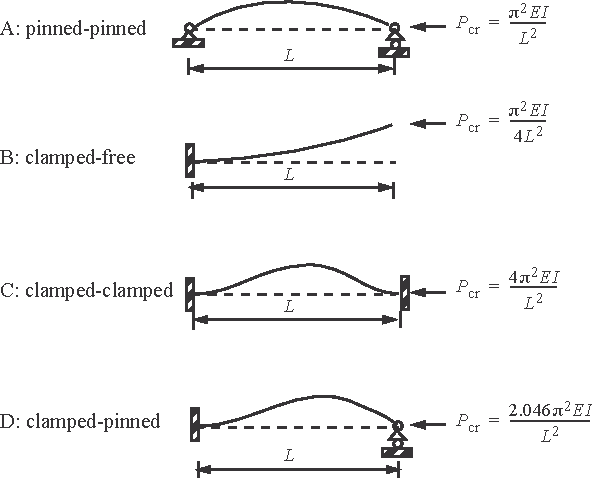
\includegraphics{Figure_11-6.pdf}}
\caption{Critical buckling loads for the standard boundary conditions A to D.} \label{fig11.6}
\vspace*{-0.8pc}
\end{figure}

\section{Initial post-buckling of the pinned-pinned column}\label{sec11.2}

The objective in this analysis is to seek an approximation for the displacement and load about the bifurcation point so that the early post-buckling behavior can be estimated. That is, does the load increase or decrease from its value at the bifurcation point on the post-buckling equilibrium path? The theory was originally due to Koiter using total potential energy (1945, in Dutch, English translation in 1970). Later Budiansky and Hutchinson (1964) and Budiansky (1966) employed the principal of virtual work to get results equivalent to Koiter's static post-buckling analysis. In this article the nonlinear equilibrium equations are used to develop the initial post-buckling behavior.

\subsection{Summary of the nonlinear equations}\label{sec11.2.1}

The overall free body diagram of the column in a deflected configuration is shown in figure~\ref{fig11.7}. The shortening of the distance between support points is denoted by $ \Delta $, where $ \Delta=-w(L) $. If the column is cut at some point along its length, then equilibrium results in the vertical force component $ S_{y}=0$ for $0 \leq z \leq L$.

The relation of the force \textit{N} to load \textit{P} is obtained from eq.~(\ref{eq11.8}) with $ H=-P $ as
\begin{align}
E A \varepsilon_{z z}+P \cos \phi=0 \label{eq11.32}
\end{align}

\begin{wrapfigure}[8]{R}{138pt}
%\vspace{-19pt}
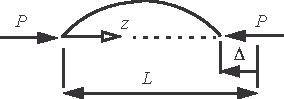
\includegraphics{Figure_11-7.pdf}
\caption{FBD of deflected pinned-pinned column. \label{fig11.7}}
\end{wrapfigure}

\noindent In eq.~(\ref{eq11.32}) force \textit{N} was replaced by Hooke's law (\ref{eq11.13}), and we dropped the subscript $x$ on the rotation $ \phi_{x} $ introduced in article~\ref{sec11.1} for convenience in the following developments. The strain $ \varepsilon_{z z} $ is related to the derivatives of the displacements by the nonlinear relation (\ref{eq11.7}). Substitute Hooke's law (\ref{eq11.13}) for the bending moment into eq.~(\ref{eq11.12}) to get the differential equation for bending as
\begin{align}\label{eq11.33}
 E I\left(\frac{d^{2} \phi}{d t^{2}}\right)-P\left(\frac{d v}{d z}\right)=0 \quad 0<z<L ,
\end{align}
From eq.~(\ref{eq11.5}) the trigonometric functions of the rotation are related to the displacements by
\begin{align}\label{eq11.34}
 \lambda \sin \phi+\frac{d v}{d z}=0 \quad \lambda \cos \phi-\left(1+\frac{d w}{d z}\right)=0 ,
\end{align}
where the stretch ratio is $ \lambda=1+\varepsilon_{z z} $. The boundary conditions to be satisfied are
\begin{align}\label{eq11.35}
 w(0)=0 \quad v(0)=\left.0 \quad \frac{d \phi}{d z}\right|_{z=0}=0 \quad v(L)=\left.0 \quad \frac{d \phi}{d z}\right|_{z=L}=0.
\end{align}

\subsection{The perturbation expansion}\label{sec11.2.2}

From the expressions in eq.~(\ref{eq11.30}) the differential equation governing buckling in terms of the rotation is
\begin{align}
E I \frac{d^{2} \phi_{1}}{d z^{2}}+P \phi_{1}=0 \quad \phi_{1}=\phi_{1}(z) \quad 0<z<L, \label{eq11.36}
\end{align}
subject to the boundary conditions
\begin{align}
\frac{d \phi_{1}}{d z}=0 \quad \text { at } \quad z=0, L. \label{eq11.37}
\end{align}
The solution to this boundary value problem is
\begin{align}
\phi_{1}(z)=-\cos \left(\frac{\pi z}{L}\right) \quad P=P_{\textrm{cr}}=\frac{\pi^{2} E I}{L^{2}}. \label{eq11.38}
\end{align}
The lateral displacement is determined from the second equation in (\ref{eq11.30}) as
\begin{align}\label{eq11.39}
 v_{1}(z)=\frac{L}{\pi} \sin \left(\frac{\pi z}{L}\right).
\end{align}

Consider the rotation and displacement in the differential equation (\ref{eq11.33}) to be a function the dimensionless parameter $ \xi $ as well as independent variable $z$ (i.e., $ \phi(\dot{z},\;\xi) $ and $ v(z,\;\xi)$). An approximate solution to the nonlinear differential equation (\ref{eq11.33}) and kinematic equation (\ref{eq11.34}) is to be determined by perturbation expansions of the dependent variables in the parameter $ \xi $ for very small values of $ \xi $. To effect the procedure, the displacements and rotation are expanded in a series in $ \xi $ as
\begin{align}\label{eq11.40}
 \begin{gathered} w(z)=w_{0}(z)+\xi w_{1}(z)+\xi^{2} w_{2}(z)+\xi^{3} w_{3}(z)+\ldots \\ v(z)=\xi v_{1}(z)+\xi^{2} v_{2}(z)+\xi^{3} v_{3}(z)+\ldots \\ \phi=\xi \phi_{1}(z)+\xi^{2} \phi_{2}(z)+\xi^{3} \phi_{3}(z)+\ldots \end{gathered}.
\end{align}
Functions $w_{0}(z)$, $\phi_{1}(z)$, and $v_{1}(z)$ are given by eqs. (\ref{eq11.14}), (\ref{eq11.38}), and (\ref{eq11.39}), respectively. The remaining functions in the expansion (\ref{eq11.40}) are to be determined. The expansion of the sine and cosine functions are
\begin{align}
\begin{gathered} \sin \phi_{x}=\sin \left[\xi \phi_{1}(z)+\xi^{2} \phi_{2}(z)+\xi^{3} \phi_{3}(z)+\ldots\right]=\xi \phi_{1}+\xi^{2} \phi_{2}+\xi^{3}\left(\phi_{3}-\frac{\phi_{x 1}^{3}}{6}\right)+O\big(\xi^{4}\big) \\
\cos \phi=\cos (\xi \phi_{1}(z)+\xi^{2} \phi_{2}(z)+\xi^{3} \phi_{3}(z)+\ldots)=1-\frac{1}{2} \xi^{2} \phi_{1}(z)-\xi^{3} \phi_{1}(z) \phi_{2}(z)+O\big(\xi^{4}\big) \end{gathered}. \label{eq11.41}
\end{align}

\subsection{Relations between the expansion functions for the rotations and lateral displacement}\label{sec11.2.3}

With respect to the discussion in article~\ref{sec11.1.3} we take $\lambda=1$, so the expansion of the first equation in (\ref{eq11.34}) is
\begin{align}\label{eq11.42}
 \xi\left[\phi_{1}+\frac{d v_{1}}{d z}\right]+\xi^{2}\left[\phi_{2}+\frac{d v_{2}}{d z}\right]+\xi^{3}\left[\phi_{3}+\frac{d v_{3}}{d z}-\frac{1}{6} \phi_{1}^{3}\right]+O\big(\xi^{4}\big)=0.
\end{align}
The previous series converges to zero for each sufficiently small value of $ \xi \neq 0 $ requires that the coefficient of each power of $ \xi $ must vanish. Hence,
\begin{align}\label{eq11.43}
 \frac{d v_{1}}{d z}=-\phi_{1} \quad \frac{d v_{2}}{d z}=-\phi_{2} \quad \frac{d v_{3}}{d z}=-\phi_{3}+\frac{1}{6} \phi_{1}^{3}.
\end{align}

\subsection{Perturbation expansion of the load \textit{P}}\label{sec11.2.4}

We utilize the relations in eq.~(\ref{eq11.43}) to get the expansion of eq.~(\ref{eq11.33}) as
\begin{align}
\xi\left(E I \frac{d^{2} \phi_{1}}{d z^{2}}+P \phi_{1}\right)+\xi^{2}\left(E I \frac{d^{2} \phi_{2}}{d z^{2}}+P \phi_{2}\right)+\xi^{3}\left(E I \frac{d^{2} \phi_{3}}{d z^{2}}+P \phi_{3}-\frac{P}{6} \phi_{1}^{3}\right)+O\big(\xi^{4}\big)=0. \label{eq11.44}
\end{align}
To determine how the load \textit{P} is a function of $\xi$ multiply eq.~(\ref{eq11.44}) by $\phi_{1}$ and integrate with respect to $z$ from $z=0$ to $z=L$:
\begin{align}
&\xi\left[\int_{0}^{L}\left(E I \frac{d^{2} \phi_{1}}{d z^{2}}+P \phi_{1}\right) \phi_{1} d z\right]+\xi^{2}\left[\int_{0}^{L}\left(E I \frac{d^{2} \phi_{2}}{d z^{2}}+P \phi_{2}\right) \phi_{1} d z\right]\nonumber\\
&\quad+\xi^{3}\left[\int_{0}^{L}\left(E I \frac{d^{2} \phi_{3}}{d z^{2}}+P \phi_{3}-\frac{P}{6} \phi_{1}^{3}\right) \phi_{1} d z\right]  +O\big(\xi^{4}\big)=0. \label{eq11.45}
\end{align}
Integrate twice by parts with respect to $z$ of the $ O\big(\xi^{2}\big)$ term in eq.~(\ref{eq11.45}) to get
\begin{align}
\int_{0}^{L} E I \frac{d^{2} \phi_{2}}{dz^{2}} \phi_{1} d z=\int_{0}^{L} E I \frac{d^{2} \phi_{1}}{dz^{2}} \phi_{2} d z+\underbrace{\left.\left[E I \frac{d \phi_{2}}{d z} \phi_{1}-E I \frac{d \phi_{1}}{d z} \phi_{2}\right]\right|_{0} ^{L}}_{=\;0}=\int_{0}^{L} E I \frac{d^{2} \phi_{1}}{dz^{2}} \phi_{2} d z. \label{eq11.46}
\end{align}
The boundary terms in the expansion functions vanish consistent with the conditions in eq.~(\ref{eq11.35}). Also, integrate twice by parts with respect to $z$ of the $ O\big(\xi^{3}\big) $ term. After integrating by parts, eq.~(\ref{eq11.45}) is
\begin{align}
&\xi\left[\int_{0}^{L}\left(E I \frac{d^{2} \phi_{1}}{d z^{2}}+P \phi_{1}\right) \phi_{1} d z\right]+\xi^{2} \int_{0}^{L}\left[\left(E I \frac{d^{2} \phi_{1}}{d z^{2}}+P \phi_{1}\right) \phi_{2} d z\right]\nonumber\\
&\quad+\xi^{3}\left[\int_{0}^{L}\left(E I \frac{d^{2} \phi_{1}}{d z^{2}}+P \phi_{1}\right) \phi_{3}-\frac{P}{6} \phi_{1}^{4} d z\right]  +O\big(\xi^{4}\big)=0. \label{eq11.47}
\end{align}
From the differential equation (\ref{eq11.36}) at buckling we have
\begin{align}
E I \frac{d^{2} \phi_{1}}{d z^{2}}=-P_{\textrm{cr}} \phi_{1}. \label{eq11.48}
\end{align}
Substitute eq.~(\ref{eq11.48}) into eq.~(\ref{eq11.47}) to find
\begin{align}
\xi\left(P-P_{c r}\right)\left(\int_{0}^{L} \phi_{1}^{2} d z\right)+\xi^{2}\left(P-P_{\textrm{cr}}\right) \int_{0}^{L} \phi_{1} \phi_{2} d z+\xi^{3}\left[\left(P-P_{\textrm{cr}}\right) \int_{0}^{L} \phi_{1} \phi_{3} d z-\frac{P}{6} \int_{0}^{L} \phi_{1}^{4} d z\right]+O\big(\xi^{4}\big)=0. \label{eq11.49}
\end{align}
The last step is to impose the orthogonality conditions on the expansion functions, which are
\begin{align}\label{eq11.50}
\int_{0}^{L} \phi_{1} \phi_{2} d z=0 \quad \int_{0}^{L} \phi_{1} \phi_{3} d z=0.
\end{align}
Equation (\ref{eq11.49}) reduces to
\begin{align}\label{eq11.51}
\xi\left(P-P_{\mathrm{cr}}\right)\left(\int_{0}^{L} \phi_{1}^{2} d z\right)-\xi^{3} \frac{P}{6} \int_{0}^{L} \phi_{1}^{4} d z+O\big(\xi^{4}\big)=0.
\end{align}
Divide eq.~(\ref{eq11.51}) by $\xi P_{\mathrm{cr}}\left(\int_{0}^{L} \phi_{1}^{2} d z\right)$ and rearrange terms to the form $\frac{P}{P_{\mathrm{cr}}}=\frac{1+O\big(\xi^{3}\big)}{\left(1-\xi^{2} b\right)}$,

\noindent where
\begin{align}\label{eq11.52}
b=\frac{1}{6}\left[\left(\int_{0}^{L} \phi_{1}^{4} d z\right) /\left(\int_{0}^{L} \phi_{1}^{2} d z\right)\right]=\frac{1}{8}.
\end{align}
The series of $\left(1-\xi^{2} b\right)^{-1}=1+b \xi^{2}+O\big(\xi^{4}\big)$, which leads to
\begin{align}\label{eq11.53}
\frac{P}{P_{\mathrm{cr}}}=1+b \xi^{2}+O\big(\xi^{3}\big).
\end{align}
In general, the expansion of $P/P_{\mathrm{cr}}$ is written as
\begin{align}\label{eq11.54}
\frac{P}{P_{\mathrm{cr}}}=1+a \xi+b \xi^{2}+\ldots.
\end{align}

\subsection{Solutions for the rotation and lateral displacement functions}\label{sec11.2.5}

Substitute the expansion of load $P$ from eq.~(\ref{eq11.54}) into eq.~(\ref{eq11.44}), and arrange terms in powers of $\xi$ to get
\begin{align}
&\xi\left[E I \frac{d^{2} \phi_{1}}{d z^{2}}+P_{\mathrm{cr}} \phi_{1}\right]+\xi^{2}\left[E I \frac{d^{2} \phi_{2}}{d z^{2}}+P_{\mathrm{cr}} \phi_{2}+a P_{\mathrm{cr}} \phi_{1}\right] \nonumber \\
&\quad +\xi^{3}\left[E I \frac{d^{2} \phi_{3}}{d z^{2}}+P_{\mathrm{cr}} \phi_{3}+a P_{\mathrm{cr}} \phi_{2}+b P_{\mathrm{cr}} \phi_{1}-\frac{1}{6} P_{\mathrm{cr}} \phi_{1}^{3}\right]+\ldots=0. \label{eq11.55}
\end{align}
For the series (\ref{eq11.55}) to converge to zero for each sufficiently small value of $\xi$, the coefficient of each power of $\xi$ must vanish. The coefficient of $\xi$ is the differential equation for buckling, eqs. (\ref{eq11.36}) and (\ref{eq11.38}). The coefficients of $\xi^{2}$ and $\xi^3$ lead to differential equations
\begin{align}\label{eq11.56}
E I \frac{d^{2} \phi_{k}}{d z^{2}}+P_{\mathrm{cr}} \phi_{k}=F_{k} \quad \phi_{k}=\phi_{k}(z) \quad 0<z<L \quad k=2,3,
\end{align}
subject to boundary conditions
\begin{align}\label{eq11.57}
\left.\frac{d\phi_{k}}{dz}\right|_{z=0}=\left.0 \quad \frac{d \phi_{k}}{d z}\right|_{z=L}=0.
\end{align}
The non-homogeneous terms in eq.~(\ref{eq11.56}) depend on previous solutions of the expansion functions. That is,
\begin{align}\label{eq11.58}
F_{2}=-a P_{\mathrm{cr}} \phi_{1} \quad F_{3}=-a P_{\mathrm{cr}} \phi_{2}-b P_{\mathrm{cr}} \phi_{1}+\frac{1}{6} P_{\mathrm{cr}} \phi_{1}^{3}.
\end{align}
Let $k_{\textrm{cr}}=P_{\textrm{cr}} /(E I)$. The general solution to differential equation (\ref{eq11.56}) consists of a complementary function $c_{1 k} \cos \left(k_{\textrm{cr}} z\right)+c_{2 k} \sin \left(k_{\textrm{cr}} z\right)$ that satisfies the homogeneous equation plus a particular solution denoted by $\phi_{k}^{*}(z)$ that satisfies the non-homogeneous equation. Then, the general solution is
\begin{align}\label{eq11.59}
\phi_{k}(z)=c_{1 k} \cos \left(k_{c r} z\right)+c_{2 k} \sin \left(k_{c r} z\right)+\phi_{k}^{*}(z).
\end{align}
Consider conditions required to solve the boundary value problem presented by eqs. (\ref{eq11.56}) and (\ref{eq11.57}). Multiply eq.~(\ref{eq11.56}) by $\phi_{1}(z)$ and integrate the result from $z=0$ to $z=L$. The result is
\begin{align}\label{eq11.60}
\int_{0}^{L}\left(E I \frac{d^{2} \phi_{k}}{d z^{2}} \phi_{1}+P_{\mathrm{cr}} \phi_{k} \phi_{1}\right) d z=\int_{0}^{L} F_{k} \phi_{1} d z.
\end{align}
Integrate the first term on the left-hand side of eq.~(\ref{eq11.60}) by parts twice to get
\begin{align}\label{eq11.61}
\left.\left[\phi_{1} E I \frac{d \phi_{k}}{d z}-\frac{d \phi_{1}}{d z} E I \phi_{k}\right]\right|_{z=L}-\left.\left[\phi_{1} E I \frac{d \phi_{k}}{d z}-\frac{d \phi_{1}}{d z} E I \phi_{k}\right]\right|_{z=0}+\int_{0}^{L}\left(E I \frac{d^{2} \phi_{1}}{d z^{2}}+P_{\mathrm{cr}} \phi_{1}\right) \phi_{k} d z=\int_{0}^{L} F_{k} \phi_{1} d z.
\end{align}
Boundary conditions (\ref{eq11.37}) and (\ref{eq11.57}) result in the terms on the left-hand side of eq.~(\ref{eq11.61}) evaluated at the end points of the interval equal to zero. Also, the integrand on the left-hand side vanishes since rotation $\phi_{1}$ satisfies eq.~(\ref{eq11.36}). We are left with the condition for the solution of the boundary value problem for $\phi_{k}$ that
\begin{align}\label{eq11.62}
\int_{0}^{L} F_{k} \phi_{1} d z=0.
\end{align}
For $k=2$ condition (\ref{eq11.62}) is
\begin{align}\label{eq11.63}
\int_{0}^{L} F_{2} \phi_{1} d z=-a P_{\mathrm{cr}} \int_{0}^{L} \phi_{1}^{2} d z=-a P_{\mathrm{cr}}\left(\frac{L}{2}\right)=0.
\end{align}
The only way to satisfy the condition in eq.~(\ref{eq11.63}) is to take the post-buckling coefficient $a=0$. The solution for $\phi_{2}$ that satisfies the boundary conditions (\ref{eq11.57}) is $\phi_{2}(z)=c_{12} \cos \left(k_{c r} z\right)$. The orthogonality condition (\ref{eq11.50}) determines $c_{12}=0$. Thus, $\phi_{2}(z)=0$. From eq.~(\ref{eq11.43}) and boundary condition (\ref{eq11.35}) we find $v_{2}(z)=0$ for ${0 \leq z \leq L}$. For $k=3$, condition (\ref{eq11.62}) is
\begin{align}\label{eq11.64}
\int_{0}^{L} F_{3} \phi_{1} d z=\int_{0}^{L}\left(-b P_{\mathrm{cr}} \phi_{1}+\frac{1}{6} P_{\mathrm{cr}} \phi_{1}^{3}\right) \phi_{1} d z=0.
\end{align}
Equation (\ref{eq11.64}) determines post-buckling coefficient $b$, and it is the same as given in eq.~(\ref{eq11.52}).
\vspace*{8pt}
\pagebreak

From eq.~(\ref{eq11.56}) the governing equation for $\phi_{3}(z)$ with $a=0$ and $b=1/8$ is
\begin{align}\label{eq11.65}
E I \frac{d^{2} \phi_{3}}{d z^{2}}+P_{\mathrm{cr}} \phi_{3}=-\left(\frac{1}{8}\right) P_{\mathrm{cr}} \phi_{1}+\frac{1}{6} P_{\mathrm{cr}} \phi_{1}^{3}=P_{\mathrm{cr}}\left[\left(\frac{1}{8}\right) \cos \left(\frac{\pi z}{L}\right)-\left(\frac{1}{6}\right) \cos ^{3}\left(\frac{\pi z}{L}\right)\right].
\end{align}
Use the trigonometric identity $\cos ^{3} x=(3/4) \cos x+(1/4) \cos (3 x)$ to find
\begin{align}\label{eq11.66}
E I \frac{d^{2} \phi_{3}}{d z^{2}}+P_{\textrm{cr}} \phi_{3}=\frac{-P_{\mathrm{cr}}}{24} \cos \left(\frac{3 \pi z}{L}\right).
\end{align}
The solution to differential equation (\ref{eq11.66}) is
\begin{align}\label{eq11.67}
\phi_{3}(z)=c_{13} \cos \left(k_{\textrm{cr}} z\right)+c_{23} \sin \left(k_{\textrm{cr}} z\right)+\left(\frac{1}{192}\right) \cos \left(\frac{3 \pi z}{L}\right).
\end{align}
Boundary conditions (\ref{eq11.57}) lead to coefficient $c_{23}=0$. Coefficient $c_{13}$ is determined from the orthogonality condition (\ref{eq11.50})\vspace*{-0.6pc}
\begin{align}\label{eq11.68}
\int_{0}^{L} \phi_{3} \phi_{1} d z=\frac{-c_{13} L}{2}=0.
\end{align}
Therefore $c_{13}=0$ and the solution for function $\phi_{3}(z)$ is
\begin{align}\label{eq11.69}
\phi_{3}(z)=\left(\frac{1}{192}\right) \cos \left(\frac{3 \pi z}{L}\right).
\end{align}
The function $v_{3}(z)$ can now be determined from eq.~(\ref{eq11.43}). The result that satisfies boundary conditions (\ref{eq11.35})~is
\begin{align}\label{eq11.70}
v_{3}(z)=\left(\frac{-L}{8 \pi}\right) \sin \left(\frac{\pi z}{L}\right)-\left(\frac{L}{64 \pi}\right) \sin \left(\frac{3 \pi z}{L}\right).
\end{align}

\subsection{Solutions for the axial displacement functions}\label{sec11.2.6}

We make use of eq.~(\ref{eq11.43}) to find that the expansion of the strain $\varepsilon_{z z}$ in (\ref{eq11.7}) is
\begin{align}\label{eq11.71}
\varepsilon_{z z}=\frac{d w_{0}}{d z}+\xi \frac{d w_{1}}{d z}+\xi^{2}\left[\frac{d w_{2}}{d z}+\frac{1}{2} \phi_{1}^{2}\right]+\xi^{3}\left[\frac{d w_{3}}{d z}+\phi_{1} \phi_{2}\right]+O\big(\xi^{4}\big).
\end{align}
Substitute expansions of the strain from eq.~(\ref{eq11.71}), the load \textit{P} from eq.~(\ref{eq11.54}), and the cosine function from eq.~(\ref{eq11.41}), into eq.~(\ref{eq11.32}) to find the expansion of the axial equilibrium as
\begin{align}\label{eq11.72}
\xi^{0}\left[E A \frac{d w_{0}}{d z}+P_{\mathrm{cr}}\right]+\xi\left[E A \frac{d w_{1}}{d z}+a P_{\mathrm{cr}}\right]+\xi^{2}\left[E A \frac{d w_{2}}{d z}+b P_{\mathrm{cr}}-P_{\mathrm{cr}} \phi_{1}^{2}+E A \frac{1}{2} \phi_{1}^{2}\right]+O\big(\xi^{3}\big)=0.
\end{align}
For eq.~(\ref{eq11.72}) to converge to zero for each sufficiently small value of $\xi$, the coefficient of each power of $\xi$ must vanish. Thus, we get to expressions for the derivatives of the expansion functions of displacement $w(z)$ as
\begin{align}\label{eq11.73}
\frac{d w_{0}}{d z}=\frac{-P_{\mathrm{cr}}}{E A} \quad \frac{d w_{1}}{d z}=\frac{-a P_{\mathrm{cr}}}{E A} \quad \frac{d w_{2}}{d z}=\frac{-2 b P_{\mathrm{cr}}+\left(2 P_{\mathrm{cr}}-E A\right) \phi_{1}^{2}}{2 E A}.
\end{align}
Since $a=0$ and $w_{1}(0)=0$, the displacement function $w_{1}(z)=0$ for $0 \leq z \leq L$. The expression for the derivative of displacement function $w_{2}(z)$ is integrated with respect to $z$, and we set $w_{2}(0)=0$ to find
\begin{align}\label{eq11.74}
w_{2}(z)=-\frac{z}{4}+\frac{7 P_{\mathrm{cr}}}{8 E A} z-\frac{L}{8 \pi} \sin \left(\frac{2 \pi z}{L}\right).
\end{align}
\vspace*{2pt}
\pagebreak

\subsection{Summary}\label{sec11.2.7}

From this initial post-buckling analysis the results for the expansions of the load, displacements, and rotation are
\begin{align}\label{eq11.75}
\frac{P}{P_{\mathrm{cr}}}=1+\frac{\xi^{2}}{8} \quad w(z)=-\frac{P_{\mathrm{cr}}}{E A} z+\xi^{2} w_{2}(z) \quad v(z)=\xi v_{1}(z)+\xi^{3} v_{3}(z) \quad \phi(z)=\xi \phi_{1}(z)+\xi^{3} \phi_{3}(z).
\end{align}
The strain of the centroidal axis is
\begin{align}\label{eq11.76}
\varepsilon_{z z}=-\frac{P_{\mathrm{cr}}}{E A}+\xi^{2}\left[\frac{d w_{2}}{d z}+\frac{1}{2}\left(\frac{d v_{1}}{d z}\right)^{2}\right].
\end{align}
Rotation functions $\phi_{1}(z)$ and $\phi_{3}(z)$ are given by eqs. (\ref{eq11.38}) and (\ref{eq11.69}), respectively. Lateral displacement functions $v_{1}(z)$ and $v_{3}(z)$ are given by eqs. (\ref{eq11.39}) and (\ref{eq11.70}), respectively, and the axial displacement function $w_{2}(z)$ is given by eq.~(\ref{eq11.74}).

\begin{example}[Numerical results for the initial post-buckling of the pinned-pinned column]\label{ex11.2}%
Consider the column with a solid, rectangular cross section of height $h$ and width $b$, where $h<b$. The radius of gyration is $r=\sqrt{I/A}=h/\sqrt{12}$. The strain at the bifurcation point is obtained from eq.~(\ref{eq11.76}) for $\xi \rightarrow 0$ is $-P_{\mathrm{cr}} /(E A)$, and take this strain equal to $-0.0006$. Since $P_{\mathrm{cr}}=\left(\pi^{2} E I\right)/ L$, we have
\begin{align}
\frac{P_{\mathrm{cr}}}{E A}=\frac{\pi^{2} E I}{L^{2}}\left(\frac{1}{E A}\right)=\frac{\pi^{2}}{12}\left(\frac{h}{L}\right)^{2}=0.0006. \label{eq11.2.a}\tag{a}
\end{align}
Hence, the span-to-thickness ratio $L/h=37$.

The restriction on the magnitude of the expansion parameter $\xi$ in the initial post-buckling analysis is based on the strain at the elastic limit of 7075-T6 aluminum alloy, which is about $0.0068$. Let $\bar{\varepsilon}_{z z}$ denote the strain of a line element parallel to the centroidal axis. It is the sum of the strain of centroidal axis $\varepsilon_{z z}$ plus the strain due to bending. That is,
\begin{align}
\bar{\varepsilon}_{z z}=\varepsilon_{z z}+y\left(\frac{d \phi}{d z}\right), \label{eq11.2.b}\tag{b}
\end{align}
where $(-h)/2 \leq y \leq h/2$ and $d \phi/d z$ is the curvature of the centroidal axis. The magnitude of the maximum compressive strain in post-buckling occurs at midspan, $z=L/2$, and $y=-h/2$. That is,
\begin{align}
\bar{\varepsilon}_{z z}=\varepsilon_{z z}-\left.\frac{h}{2}\left(\frac{d \phi}{d z}\right)\right|_{z=L/2}. \label{eq11.2.c}\tag{c}
\end{align}
The expansion for the curvature at midspan is determined from eqs. (\ref{eq11.75}), (\ref{eq11.38}) and (\ref{eq11.69}). The result is
\begin{align}
\left.\frac{d \phi}{d z}\right|_{z=L/2}=\left[\frac{\pi}{L} \sin \left(\frac{\pi z}{L}\right)\right] \xi-\left.\left[\frac{\pi}{64 L} \sin \left(\frac{3 \pi z}{L}\right)\right] \xi^{3}\right|_{z=L/2}=\frac{\pi}{L} \xi+\frac{\pi}{64 L} \xi^{3}. \label{eq11.2.d}\tag{d}
\end{align}
Substitute $h=0.270L$ and $P_{\mathrm{cr}}=0.0006 \mathrm{EA}$ in the expansions for the strains. The numerical evaluations of the strain in eq.~(\ref{eq11.76}) and the strain from bending are
\begin{align}
\varepsilon_{z z}=-0.0006-0.000075 \xi^{2} \quad-\frac{h}{2}\left(\frac{d \phi}{d z}\right)=-0.0424264 \xi-0.000662193 \xi^{3}. \label{eq11.2.e}\tag{e}
\end{align}
The axial strain on the concave side of the bar at midspan is set equal to the elastic limit strain of $-0.0068$. Thus,
\begin{align*}
\bar{\varepsilon}_{z z}=-0.0006-0.042464 \xi-0.000075 \xi^{2}-0.000662913 \xi^{3}=-0.0068.
\end{align*}
The real root of the previous polynomial is the maximum value of parameter $\xi$, which is
\begin{align}
\xi_{\max }=0.14605. \label{eq11.2.f}\tag{f}
\end{align}
For post-buckling coefficients $a=0$ and $b=1/8$, we get $P/P_{\mathrm{cr}}=1.0027$ at $\xi=\xi_{\max}$ from eq.~(\ref{eq11.54}). There is a very small increase in the load during post-buckling. The lateral displacement of the column is determined from eqs. (\ref{eq11.75}), (\ref{eq11.39}), and (\ref{eq11.70}), and it is a maximum at midspan. Evaluation of the maximum displacement is
\begin{align}
v_{\max }=v(L/2)=\frac{L \xi}{\pi}-\frac{7 L \xi^{2}}{64 \pi}, \label{eq11.2.g}\tag{g}
\end{align}
and $v_{\max }=0.04638\,{L}$ at $\xi=\xi_{\max }$.

The axial displacement of the column is determined from eqs. (\ref{eq11.75}) and (\ref{eq11.74}). The shortening of distance between supports is
\begin{align}
\Delta=-w(L)=L(0.0006)+\left(\frac{L}{4}+\frac{L(0.0006)}{8}\right) \xi^{2}. \label{eq11.2.h}\tag{h}
\end{align}
The shortening at buckling is $\Delta_{\mathrm{cr}}=\left.\Delta\right|_{\xi=0}=L(0.0006)$, and the normalized shortening is defined by
\begin{align}
\Delta/\Delta_{\mathrm{cr}}=1+416.792 \xi^{2}. \label{eq11.2.i}\tag{i}
\end{align}
At $\xi=\xi_{\max }$, $\Delta/\Delta_{\mathrm{cr}}=9.89$ on the post-buckling path. The configuration of the column at $\xi_{\max }$ is shown in figure~\ref{fig11.8}.

\processfigure{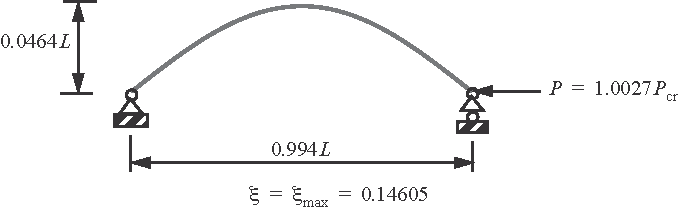
\includegraphics{Figure_11-8.pdf}}{\caption{Post-buckling configuration of the pinned-pinned column at the elastic limit strain.}\label{fig11.8}}

The pre-buckling equilibrium path is determined from eq.~(\ref{eq11.14}) where $\Delta=-w_{0}(L)=(P L) /(E A)$, or ${P=(E A/ L) \Delta}$. Divide by the critical load to get $P/P_{\mathrm{cr}}=\left(E A/P_{\mathrm{cr}}\right)(\Delta/L)$. From eq. (\textbf{\ref{eq11.2.a}}) the factor $E A/P_{\mathrm{cr}}=1/0.0006$. Thus, $P/P_{\mathrm{cr}}=\Delta /(0.0006 L)=\Delta/ \Delta_{\mathrm{cr}}$ on the pre-buckling equilibrium path.

\begin{figure}[!h]
\centerline{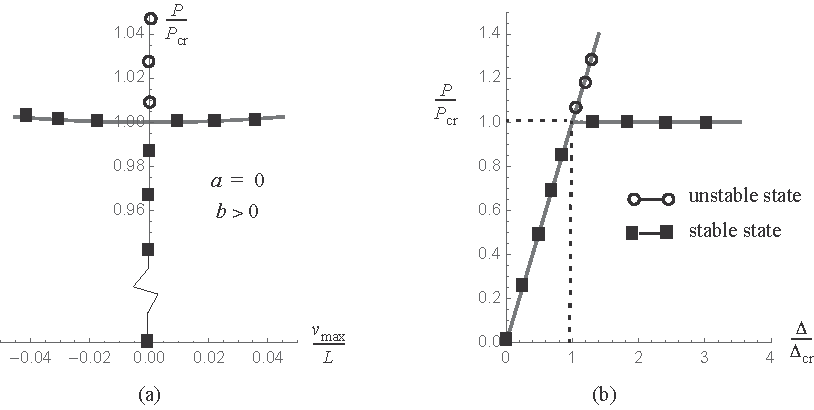
\includegraphics{Figure_11-9.pdf}}
\caption{Equilibrium paths for the pinned-pinned column subject to axial compression (a) on the load-deflection plot, and (b) on the load-shortening plot.} \label{fig11.9}
\end{figure}

 The load-deflection response is shown in figure~\ref{fig11.9}(a), and the load-shortening response is shown in figure~\ref{fig11.9}(b). The post-buckling behavior of the column is \textbf{stable symmetric bifurcation}, which is the same behavior as model~A in article~\ref{sec10.1} on page~\pageref{sec10.1}. The load does not decrease in post-buckling. However, the increase in load is very small in post-buckling. From a practical point of view, the column is considered\vadjust{\vspace*{8pt}\pagebreak} neutral in post-buckling.The structural stiffness is defined as $d P/d \Delta$. For post-buckling the structural stiffness is computed~as
\begin{align*}
\frac{d P}{d \Delta}=\frac{d P}{d \xi} \frac{d \xi}{d \Delta}=\left(\frac{P_{\mathrm{cr}}}{4} \xi\right) \frac{1}{2(L/ 4+0.0006(L/8)) \xi}=\frac{P_{\mathrm{cr}}}{L(2+0.0006)}=\frac{E A(0.0006)}{L(2.0006)}=\frac{E A}{L}(0.0003).
\end{align*}
The structural stiffness in pre-buckling is $(E A)/L$. The ratio of the post-buckling stiffness to the pre-buckling stiffness is 0.0003, which indicates the dramatic loss of structural stiffness due to buckling.
\end{example}

From eq.~(\ref{eq11.54}) the perturbation expansion of the load in initial post-buckling is $P/P_{\mathrm{cr}}=1+a \xi+b \xi^{2}$. The post-buckling coefficients $a=0$ and $b<0$ correspond to unstable symmetric bifurcation behavior illustrated by model B in article~\ref{sec10.2} on page~\pageref{sec10.2}. Post-buckling coefficient $a \neq 0$ corresponds to asymmetric bifurcation behavior illustrated by model C in article~\ref{sec10.3} on page~\pageref{sec10.3}.

\section{In-plane buckling of trusses}\label{sec11.3}

When a truss has all of its joints pinned, then there will be no interaction between the bending deflections of individual members. Hence the buckling load of the truss will be the load at which the weakest compression member buckles as an Euler column (case A in figure~\ref{fig11.6}). However, when a truss is rigidly jointed, as in a frame, there will be interaction between bending deflections of neighboring members through rotation of the common joint. A rigid-jointed truss is stiffer than a pin-jointed truss, and therefore its buckling load is increased relative to the pin-jointed truss.

\begin{example}[Buckling of a two-bar truss]\label{ex11.3}%
A symmetric truss consisting of two identical bars of length \textit{L} are connected together by a hinge joint at the center of the truss. The opposite end of each bar connects to a separate hinge joint at a fixed support.\vadjust{\vspace*{8pt}\pagebreak} Both supports are at a distance \textit{H} below central joint. The central joint is subject to downward load \textit{Q} whose corresponding displacement is denoted by $q$.

We consider a linear analysis and a nonlinear analysis for the stability of the truss, where Hooke's law governs the material behavior in both analyses. The material of the bars is 7075-T6 aluminum alloy with a modulus of elasticity $E=71{,}000\,\mathrm{N}/\mathrm{mm}^{2}$ and yield strength of $\sigma_{\text {yield }}=469\,\textrm{MPa}$. The remaining numerical data are listed in table~\ref{tab11.2}. From the data in table~\ref{tab11.2} the angle $\beta=5.16^{\circ}$. A small value of $\beta$ characterizes a shallow truss configuration.

\begin{figure}[!h]
\centerline{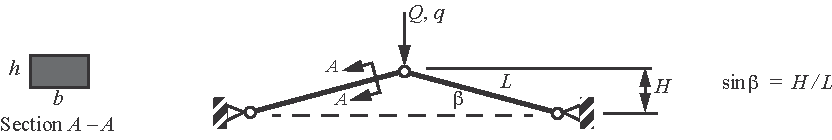
\includegraphics{Figure_11-10.pdf}}
\caption{A shallow truss horizontally constrained between fixed points.} \label{fig11.10}
\end{figure}

\begin{table}[!h]
\processtable{Numerical data for the truss in figure~\ref{fig11.10} \label{tab11.2}}{
\tabcolsep=11pt\begin{tabular}{@{}llll@{}}
\toprule
Length of truss bars \textit{L},\,mm & 300 & Width of truss bar $b$,\,mm & \phantom{12,0}25 \\
Truss rise above supports \textit{H},\,mm & \phantom{0}27 & Area of truss bar \textit{A},\,mm$^{2}$ & \phantom{12,}450 \\
Thickness of truss bar $h$,\,mm & \phantom{0}18 & Second area moment \textit{I},\,mm$^{4}$ & 12,150 \\
\botrule
\end{tabular}}{}
\vspace*{-1pc}
\end{table}

\subsubsection{Axial strain-displacement relation.} The strain-displacement relation (\ref{eq11.7}) for each bar is
\begin{align}
\varepsilon_{z z}=\frac{d w}{d z}+\frac{1}{2}\left(\frac{d v}{d z}\right)^{2}, \label{eq11.3.a}\tag{a}
\end{align}

\vspace*{-1pc}

\begin{wrapfigure}[10]{L}{122pt}
\vspace{-19pt}
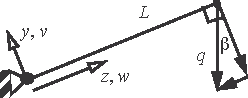
\includegraphics{Figure_11-11.pdf}
\caption{Left-hand bar of the truss.\label{fig11.11}}
\end{wrapfigure}

\noindent where the axial displacement is denoted by $w(z)$ and the lateral displacement is denoted by $v(z)$. Consider the bar on the left-hand side of the truss as shown in figure~\ref{fig11.11}. At the fixed end where $z= 0$, $w(0)=v(0)=0$. At the end of the bar where $z=L$ the axial displacement and the lateral displacement are related to the downward displacement $q$ of the movable joint by $w(L)=-q \sin \beta$ and $v(L)=-q \cos \beta$, respectively. The axial strain in a truss bar is uniform along its length, which means that the displacements are linear in coordinate $z$. Linear displacement functions for each displacement satisfying the end conditions are,
\begin{align}
w(z)=(-q \sin \beta)(z/L) \quad v(z)=(-q \cos \beta)(z/L). \label{eq11.3.b}\tag{b}
\end{align}
Substitute eq. (\textbf{\ref{eq11.3.b}}) for the displacement functions into eq. (\textbf{\ref{eq11.3.a}}) to get the strain-displacement relation
\begin{align}
\varepsilon_{z z}=(\sin \beta)\left(\frac{-q}{L}\right)+\frac{1}{2}\left(\cos ^{2} \beta\right)\left(\frac{q}{L}\right)^{2}. \label{eq11.3.c}\tag{c}
\end{align}
Substitute $\sin \beta=H/L$, and $\cos \beta=\big(\sqrt{L^{2}-H^{2}}\big)/L$ into eq. (\textbf{\ref{eq11.3.c}}) to get
\begin{align}
\varepsilon_{z z}=\frac{H}{L}\left(\frac{-q}{L}\right)+\frac{\left(L^{2}-H^{2}\right)}{2 L^{2}}\left(\frac{-q}{L}\right)^{2}. \label{eq11.3.d}\tag{d}
\end{align}
Numerical evaluation of eq. (\textbf{\ref{eq11.3.d}}) is
\begin{align}
\varepsilon_{z z}=\left(-3 \times 10^{-4}/\mathrm{mm}\right) q+\left(5.51056 \times 10^{6}/\mathrm{mm}^{2}\right) q^{2}. \label{eq11.3.e}\tag{e}
\end{align}
The strain energy of the truss is\vspace*{-0.6pc}
\begin{align}
U=2\left(\frac{1}{2} E A L \varepsilon_{z z}^{2}\right), \label{eq11.3.f}\tag{f}
\end{align}
in which the leading factor of 2 accounts for the two bars. Castigliano's first theorem determines the force \textit{Q} by
\begin{align}
Q=\frac{\partial U}{\partial q}=2 E A L \varepsilon_{z z} \frac{\partial \varepsilon_{z z}}{\partial q}. \label{eq11.3.g}\tag{g}
\end{align}
Substitute eq. (\textbf{\ref{eq11.3.d}}) for the strain into eq. (\textbf{\ref{eq11.3.f}}) to get
\begin{align}
Q=2 E A\left[\frac{H^{2}}{L^{3}} q-\frac{3 H\left(L^{2}-H^{2}\right)}{2 L^{5}} q^{2}+\frac{\left(L^{2}-H^{2}\right)^{2}}{2 L^{7}} q^{3}\right]. \label{eq11.3.h}\tag{h}
\end{align}
Numerical evaluation of eq. (\textbf{\ref{eq11.3.h}}) is
\begin{align}
Q=(1{,}725.3\,\mathrm{N}/\mathrm{mm}) q-(95.0736\,\mathrm{N}/\mathrm{mm}^{2}) q^{2}+(1.16424\,\mathrm{N}/ \mathrm{mm}^{3}) q^{3}. \label{eq11.3.i}\tag{i}
\end{align}

\vspace*{-1pc}

\subsubsection{In-plane buckling of the truss bars based on linear analysis.} The expressions for the axial strain (\textbf{\ref{eq11.3.e}}) and applied load (\textbf{\ref{eq11.3.h}}) reduce to
\begin{align}
\varepsilon_{z z}=\frac{H}{L}\left(\frac{-q}{L}\right)=(-3 \times 10^{-4}\,\mathrm{mm}^{-1}) q,\,\textrm{and } Q=2 E A\left[\frac{H^{2}}{L^{3}} q\right]=(1{,}725.3\,\mathrm{N}/\mathrm{mm}) q. \label{eq11.3.j}\tag{j}
\end{align}
The axial force in each bar is given by
\begin{align}
N=E A \varepsilon_{z z}=(-9{,}585\,\mathrm{N}/\mathrm{mm}) q. \label{eq11.3.k}\tag{k}
\end{align}
The Euler buckling force $P_{E}=\left(\pi^{2} E I\right)/L^{2}=94.60\,\textrm{kN}$. Set $-N=P_{E}$ to find the displacement for in-plane buckling of the truss bars $q=9.87\,\mathrm{mm}$. The corresponding load $Q=17.028\,\textrm{kN}$.

Equations (\textbf{\ref{eq11.3.i}}) and (\textbf{\ref{eq11.3.j}}) are plotted on the graph of load \textit{Q} versus displacement $q$ in figure~\ref{fig11.12}. As the load is increased from zero on the nonlinear path (\textbf{\ref{eq11.3.i}}) a \textbf{limit point} load of 9.038~kN at a displacement of 11.5~mm is encountered. As discussed in article~\ref{sec10.5} a dynamic snap-through motion occurs at the limit load that eventually (with damping) settles to a displacement of 58.65~mm. The linear response path (\textbf{\ref{eq11.3.j}}) is the straight line in figure~\ref{fig11.12}, and the load causing in-plane buckling of the truss bars is 17.028~kN. Thus, the critical load for this structure is at the limit point.
\end{example}

\section{Geometrically imperfect column}\label{sec11.4}

Consider a uniform, pinned-pinned column that is slightly crooked under no load. The initial shape under no load is described by the function $v_{0}(z)$. The column is subject to a centric, axial compressive load \textit{P}. The lateral displacement of the column is denoted by $v(z)$, so that $v(z)=v_{0}(z)$ when $P=0$. Moment equilibrium of the\vadjust{\vspace*{8pt}\pagebreak} free body diagram for a segment of the column shown in figure~\ref{fig11.13} is
\begin{align}\label{eq11.77}
M_{x}-v P=0.
\end{align}

\begin{figure}[!t]
\centerline{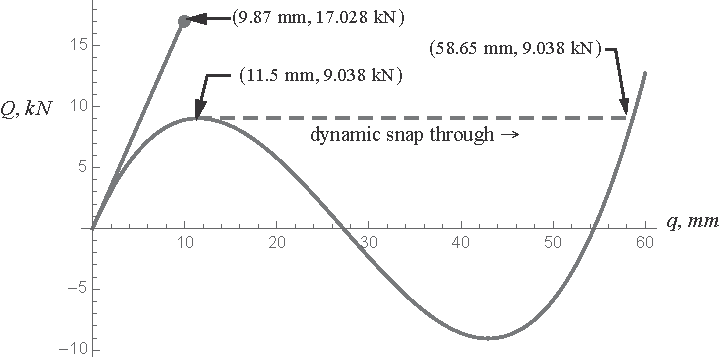
\includegraphics{Figure_11-12.pdf}}
\caption{Load-displacement responses of the two-bar truss from linear and nonlinear analyses.} \label{fig11.12}
\vspace{-6pt}
\end{figure}

\begin{wrapfigure}[8]{L}{108pt}
\vspace{-19pt}
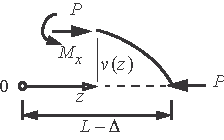
\includegraphics{Figure_11-13.pdf}
\caption{FBD of the right-hand part of a pinned-pinned column.\label{fig11.13}}
\end{wrapfigure}

\vspace*{-1pc}

\noindent The bending moment in the column is zero under no load, so we write the material law for bending as\vspace*{-6pt}
\begin{align}\label{eq11.78}
M_{x}=E I\left(\frac{d \phi}{d z}-\frac{d \phi_{0}}{d z}\right),
\end{align}
where $\phi_{0}(z)$ is the rotation of the initial shape of the column. For small slopes of the slightly deflected column the rotations are related to the lateral displacements~by
\begin{align}
\phi(z)=-\left(\frac{d v}{d z}\right) \quad \phi_{0}(z)=-\left(\frac{d v_{0}}{d z}\right). \label{eq11.79}
\end{align}
Hence, the bending moment becomes
\begin{align}\label{eq11.80}
M_{x}=-E I\left(\frac{d^{2} v}{d z^{2}}-\frac{d^{2} v_{0}}{d z^{2}}\right).
\end{align}
Substitute the bending moment from eq.~(\ref{eq11.80}) into the moment equilibrium equation (\ref{eq11.77}) to get
\begin{align}\label{eq11.81}
-E I\left(\frac{d^{2} v}{d z^{2}}-\frac{d^{2} v_{0}}{d z^{2}}\right)-v P=0.
\end{align}




\noindent Equation (\ref{eq11.81}) is arranged to the form
\begin{align}\label{eq11.82}
\frac{d^{2} v}{d z^{2}}+k^{2} v=\frac{d^{2} v_{0}}{d z^{2}},
\end{align}
where $k^{2}=P /(E I)$. Take the initial shape of the column $v_{0}(z)=a_{1} \sin (\pi z/L)$, where $a_1$ is the amplitude of the initial shape at midspan. Then the differential equation for $v(z)$ is
\begin{align}\label{eq11.83}
\frac{d^{2} v}{d z^{2}}+k^{2} v=-a_{1}\left(\frac{\pi}{L}\right)^{2} \sin (\pi z/L) \quad 0<z<L.
\end{align}
The boundary conditions are $v(0)=v(L)=0$. The solution of the differential equation (\ref{eq11.83}) subject to boundary conditions is
\begin{align}\label{eq11.84}
v(z)=\frac{a_{1}}{1-\left(\frac{k L}{\pi}\right)^{2}} \sin \left(\frac{\pi z}{L}\right) \quad 0 \leq z \leq L.
\end{align}
The term $k^{2} L^{2}/\pi^{2}=P/P_{\mathrm{cr}}$ where the critical load of the perfect structure is $P_{\mathrm{cr}}=\left(\pi^{2} E I\right)/L^{2}$. It is convenient to measure the deflection of the imperfect column under load with respect to its original unloaded state. That is, let $\delta$ define the additional displacement at midspan by $\delta=v(L/2)-v_{0}(L/2)$. Hence,
\begin{align}\label{eq11.85}
\delta=a_{1} \frac{\left(\frac{P}{P_{\textrm{cr}}}\right)}{1-\left(\frac{P}{P_{\textrm{cr}}}\right)}.
\end{align}
The load-displacement response is sketched in figure~\ref{fig11.14}. Note that $|\delta| \rightarrow \infty$ as $P \rightarrow P_{\mathrm{cr}}$ for $a_{1} \neq 0$. That is, for a non-zero value of the imperfection amplitude, the displacement gets very large as the axial force approaches the buckling load of the perfect column. Also, the imperfect column deflects in the direction of imperfection (e.g., if $a_{1}>0$, then $\delta>0$).

\processfigure{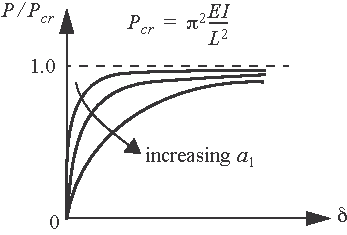
\includegraphics{Figure_11-14.pdf}}{\caption{Load-deflection response plots for geometrically imperfect columns.}\label{fig11.14}}

An arbitrary initial shape is represented by a Fourier Sine series as
\begin{align}\label{eq11.86}
v_{0}(z)=a_{1} \sin \frac{\pi z}{L}+a_{2} \sin \frac{2 \pi z}{L}+\ldots.
\end{align}
Timoshenko and Gere (1961) show the solution for $\delta(z)=v(z)-v_{0}(z)$ is
\begin{align}\label{eq11.87}
\delta(z)=\frac{P}{P_{\mathrm{cr}}}\left[\frac{a_{1}}{1-P/P_{\mathrm{cr}}} \sin \left(\frac{\pi z}{L}\right)+\frac{a_{2}}{2^{2}-P/P_{\mathrm{cr}}} \sin \left(\frac{2 \pi z}{L}\right)+\ldots\right].
\end{align}
For $P<P_{\mathrm{cr}}$ as $P \rightarrow P_{\mathrm{cr}}$, the first term dominates the solution for $\delta(z)$. Thus, for \textit{P} near $P_{\textrm{cr}}$
\begin{align}\label{eq11.88}
\delta_{c}=\delta\left(\frac{L}{2}\right) \sim \frac{P/P_{\textrm{cr}}}{1-P/P_{\textrm{cr}}} a_{1}.
\end{align}

\vspace*{-1pc}

The buckling behavior of a long, straight column subject to centric axial compression (the perfect column) is classified as stable symmetric bifurcation. As such it is imperfection insensitive. Refer to the discussions in article~\ref{sec10.1.5} on page~\pageref{sec10.1.5} and article~\ref{sec10.2.1} on page~\pageref{sec10.2.1}. Even for a well manufactured column whose geometric imperfections are small, and with the load eccentricity small, the displacements become excessive as the axial compressive force $P$ approaches the critical load $P_{\textrm{cr}}$ of the perfect column. \textit{Hence, the critical load determined from the analysis of the perfect column is meaningful in practice}\vadjust{\vspace*{8pt}\pagebreak}.

\subsection{Southwell plot}\label{sec11.4.1}

Rearrange eq.~(\ref{eq11.88}) as follows: $\delta_{c}\left(1-P/P_{\textrm{cr}}\right)=\left(P/P_{\textrm{cr}}\right) a_{1}$, then $\delta_{c}-\left(P/P_{\textrm{cr}}\right) \delta_{c}=\left(P/P_{\textrm{cr}}\right) a_{1}$. Divide the last by \textit{P} to get
\begin{align}
\frac{\delta_{c}}{P}=\frac{\left(\delta_{c}+a_{1}\right)}{P_{\textrm{cr}}}. \label{eq11.89}
\end{align}
We plot $\delta_{c}/P$ versus $\delta_{c}$ from eq.~(\ref{eq11.89}) in figure~\ref{fig11.15}, which is called the Southwell plot (Southwell, 1932).\footnote{Richard V. Southwell (1888--1970), British mathematician specializing in applied mechanics. In his article ``On the Analysis of Experimental Observations in Problems of Elastic Stability'', he discussed the coordinates used in the plot to correlate the experimental data on elastic column buckling with linear theory.} The Southwell plot is very useful for determining $P_{\textrm{cr}}$ from test data in the elastic range. As $P \rightarrow P_{\textrm{cr}}$, $P<P_{\textrm{cr}}$, $\delta$ becomes large and the data ($(\delta/P) \text { vs. } \delta$) tends to plot on a straight line. Extrapolating this straight line back to toward the ordinate axis ($\delta/P$) one can estimate $a_1$ and $P_{\textrm{cr}}$. It is more difficult to determine $P_{\textrm{cr}}$ by the load-deflection curve obtained in experiments as illustrated in figure~\ref{fig11.16}.

\processfigure{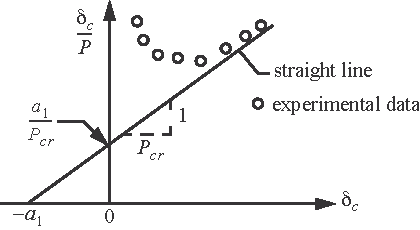
\includegraphics{Figure_11-15.pdf}}{\caption{Southwell plot.}\label{fig11.15}}

\processfigure{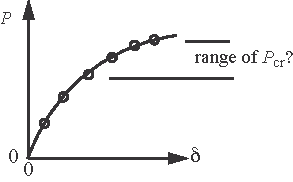
\includegraphics{Figure_11-16.pdf}}{\caption{Load-deflection plot from test data.}\label{fig11.16}}

\vspace*{-1pc}

\section{Column design curve}\label{sec11.5}

Consider the pinned-pinned uniform column whose critical load is given by $P_{\textrm{cr}}=\pi^{2}\left(E I/L^{2}\right)$. Let \textit{A} denote the cross-sectional area of the column. At the onset of buckling the critical stress is defined as%\vspace*{-6pt}
\begin{align}\label{eq11.90}
\sigma_{\textrm{cr}}=P_{\textrm{cr}}/A=\left(\pi^{2} E I\right) /\left(A L^{2}\right).
\end{align}

\begin{wrapfigure}[6]{R}{70pt}
%\vspace{-19pt}
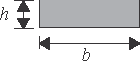
\includegraphics{Figure_11-17.pdf}
\caption{ \label{fig11.17}}
\end{wrapfigure}

\vspace*{-1pc}

\noindent The second area moment is $I=r^{2} A$, where $r$ denotes the minimum radius of gyration of the cross section. For the rectangular section shown in figure~\ref{fig11.17}, $I_{\min}=\big(b h^{3}\big)/12$ and $A=b h$, so that $r=h/ \sqrt{12}$, where $0<h<b$. Thus, the critical stress becomes
\begin{align}\label{eq11.91}
\sigma_{\textrm{cr}}=\pi^{2} \frac{E}{(L/r)^{2}}.
\end{align}
and $L/r$ is called the \textit{slenderness ratio}. The slenderness ratio is the column length divided by a cross-sectional dimension significant to bending.

For any set of boundary conditions define the \textit{effective length} $K L$ by the formula
\begin{align}\label{eq11.92}
P_{\textrm{cr}}=\pi^{2} \frac{E I}{(K L)^{2}}.
\end{align}
The effective lengths for the four standard boundary conditions are as follows:
\begin{align*}
\begin{array}{llll}
\textrm{A: pinned-pinned } &\quad P_{\textrm{cr}}=\pi^{2} \dfrac{E I}{L^{2}}=\pi^{2} \frac{E I}{(K L)^{2}}&\quad K L=L&\quad K=1 \\[6pt]
\textrm{B: clamped-free }&\quad P_{\textrm{cr}}=\frac{\pi^{2}}{4}\dfrac{E I}{L^{2}}=\pi^{2} \frac{E I}{(K L)^{2}}&\quad K L=2 L&\quad K=2\\[6pt]
\textrm{C: clamped-clamped }&\quad P_{\textrm{cr}}=4 \pi^{2} \dfrac{E I}{L^{2}}=\pi^{2} \frac{E I}{(K L)^{2}}&\quad K L=L/2&\quad K=1/2 \\[6pt]
\textrm{D: clamped-pinned }&\quad P_{\textrm{cr}}=20.2 \dfrac{E I}{L^{2}}=\pi^{2} \frac{E I}{(K L)^{2}}&\quad KL=0.699~L&\quad K=0.7
\end{array}
\end{align*}
The definition of effective length uses case A boundary conditions as a reference. The concept of effective length accounts for boundary conditions other than simple support, or pinned-pinned end conditions.

The \textit{column curve} is a plot of the critical stress versus the effective slenderness ratio (i.e., $\sigma_{cr} \text { versus } K L/r$). For elastic column buckling under all boundary conditions
\begin{align}\label{eq11.93}
\sigma_{\textrm{cr}}=\frac{\pi^{2} E}{\left(\frac{K L}{r}\right)^{2}},
\end{align}
which is a hyperbola that depends only on the modulus of elasticity \textit{E} of the material. This equation governing elastic buckling is called the Euler curve, and columns that buckle in the elastic range are called long columns. See figure~\ref{fig11.18}.

\processfigure{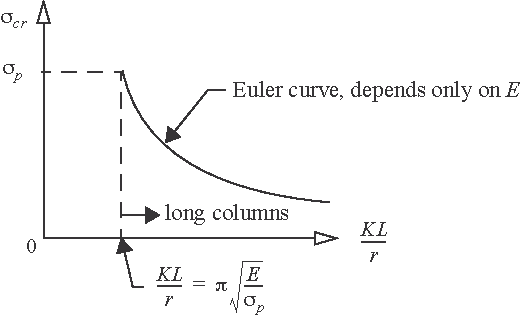
\includegraphics{Figure_11-18.pdf}}{\caption{Column curve for elastic buckling.}\label{fig11.18}}


\subsection{Inelastic buckling}\label{sec11.5.1}

The column curve equation, eq.~(\ref{eq11.93}), is valid up to the proportional limit of the material, denoted by $\sigma_{p}$. The proportional limit is defined as the stress where the compressive stress-strain curve of the material deviates from a straight line. If the stress at the onset of buckling is greater than the proportional limit, then the column is said to be of intermediate length, and the Euler formula, eq.~(\ref{eq11.93}), cannot be used. The proportional limit is difficult to measure from test data because its definition is based on the deviation from linearity. In particular, the compressive stress-strain curves for aluminum alloys typically used in aircraft construction do not exhibit a\vadjust{\vspace*{8pt}\pagebreak} very pronounced linear range. For aluminum alloys a material law developed by Ramberg and Osgood (1943) is often used to describe the nonlinear compressive stress-strain curve. The Ramberg-Osgood equation is a three-parameter fit to the compressive stress-strain curves of aluminum alloys. From the experimental compressive stress-strain curve the slope near the origin is the modulus of elasticity \textit{E}. The stress where the secant line drawn from the origin with slope 0.85~\textit{E} intersects the stress-strain curve is denoted $\sigma_{0.85}$.The stress where a second secant line drawn from the origin with slope 0.7~\textit{E} intersects the stress-strain curve is denoted by $\sigma_{0.7}$. These data are depicted in figure~\ref{fig11.19}. Note that the compressive normal strain corresponding to the stress $\sigma_{0.7}$ is usually about the 0.2 percent offset yield strain for the material. Hence, stress $\sigma_{0.7}$ is close to the 0.2 percent offset yield stress of the aluminum alloy. The Ramberg-Osgood equation is

\processfigure[!h]{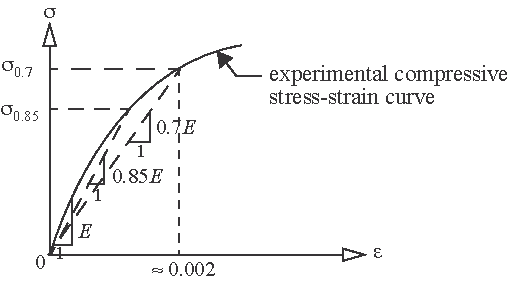
\includegraphics{Figure_11-19.pdf}}{\caption{Data used to fit the compression stress-strain curve of aluminum alloys.}\label{fig11.19}}

\vspace*{-1pc}

\begin{align}\label{eq11.94}
\varepsilon=\frac{\sigma}{E}\left[1+\frac{3}{7}\left(\frac{\sigma}{\sigma_{0.7}}\right)^{n-1}\right],
\end{align}
where the shape parameter $n$ is given by
\begin{align}\label{eq11.95}
n=1+\ln \left(\frac{17}{7}\right)/\ln \left(\frac{\sigma_{0.7}}{\sigma_{0.85}}\right).
\end{align}
Equation (\ref{eq11.94}) is re-written as
\begin{align}\label{eq11.96}
\frac{E \varepsilon}{\sigma_{0.7}}=\frac{\sigma}{\sigma_{0.7}}+\frac{3}{7}\left(\frac{\sigma}{\sigma_{0.7}}\right)^{n},
\end{align}

\vspace*{-0.6pc}

\noindent and is plotted as $\sigma/\sigma_{0.7}$ versus $(E \varepsilon)/\sigma_{0.7}$ for various values of the shape parameter $n$, This plot is shown in figure~\ref{fig11.20}. Some approximate values for common aluminum alloys are listed in table~\ref{tab11.3}.

\begin{table}[!h]
\processtable{Ramberg-Osgood parameters for selected aluminum alloys \label{tab11.3}}{%
\tabcolsep=36pt\begin{tabular}{@{}llll@{}}
\toprule
\colhead{\textit{AL}} & \colhead{\textit{E} in 10$^{\textbf{6}}$ psi} & \colhead{$\boldsymbol{\sigma}_{\textbf{0.7}}$ in 10$^{\textbf{3}}$psi} & \colhead{\textbf{$n$}} \\
\midrule
2014-T6 & 10.6 & 60 & 20 \\
2024-T4 & 10.6 & 48 & 10 \\
6061-T6 & 10.0 & 40 & 30 \\
7075-T6 & 10.4 & 73 & 20 \\
\botrule
\end{tabular}}{}
\vspace*{-1pc}
\end{table}

\begin{figure}[!h]
\centerline{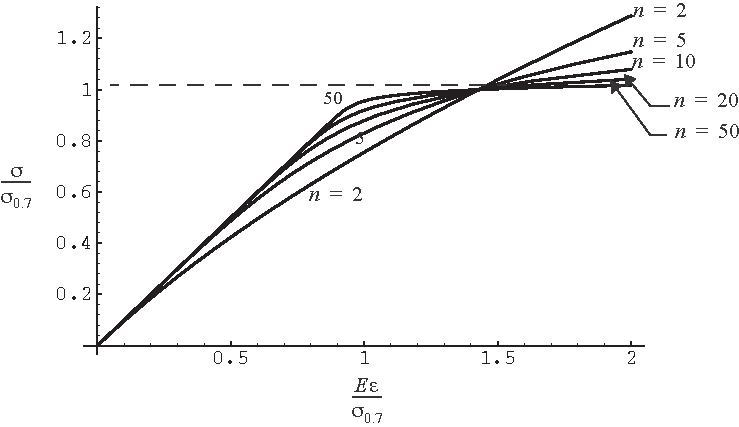
\includegraphics{Figure_11-20.pdf}}
\caption{A normalized plot of the Ramberg-Osgood material law for various values of the shape parameter $n$.} \label{fig11.20}
\end{figure}

From the Ramberg-Osgood equation, eq.~(\ref{eq11.94}), the local slope of the compressive stress-strain curve is determined as a function of the stress. This slope of the compressive stress-strain curve is called the tangent modulus (i.e., $\frac{d \sigma}{d \varepsilon}=E_{t}$ where $E_t$ is the tangent modulus). Differentiate eq.~(\ref{eq11.94}) to\vspace*{-3pt} get
\begin{align}\label{eq11.97}
d \varepsilon=\frac{d \sigma}{E}+\frac{3}{7} \frac{n \sigma^{n-1}}{E \sigma_{0.7}^{n}-1} d \sigma \quad \frac{d \varepsilon}{d \sigma}=\frac{1}{E_{t}}=\frac{1}{E}+\frac{3}{7} \frac{n}{E}\left(\frac{\sigma}{\sigma_{0.7}}\right)^{n-1}.
\end{align}
Thus, the tangent modulus\vspace*{-3pt} is
\begin{align}\label{eq11.98}
E_{t}=\frac{E}{1+\frac{3}{7} n\left(\frac{\sigma}{\sigma_{0.7}}\right)^{n-1}}.
\end{align}

\removelastskip

For intermediate length columns it has been demonstrated by extensive testing that the critical stress is reasonably well predicted using the Euler curve, eq.~(\ref{eq11.93}), with the modulus of elasticity replaced by the tangent modulus. This inelastic buckling analysis is called the \textit{tangent modulus theory}. That is\vspace*{-3pt},
\begin{align}\label{eq11.99}
\sigma_{\textrm{cr}}=\pi^{2} \frac{E_{t}}{\left(\frac{K L}{r}\right)^{2}}.
\end{align}
Now substitute eq.~(\ref{eq11.98}) for the tangent modulus in the latter equation, noting that $\sigma=\sigma_{\textrm{cr}}$, to\vspace*{-3pt} get
\begin{align}\label{eq11.100}
\sigma_{\textrm{cr}}=\frac{\pi^{2}}{\left(\frac{K L}{r}\right)^{2}}\left[\frac{E}{1+\frac{3}{7} n\left(\frac{\sigma_{\textrm{cr}}}{\sigma_{0.7}}\right)^{n-1}}\right].
\end{align}
After division by $\sigma_{0.7}$, eq.~(\ref{eq11.100}) can be written as
\begin{align}\label{eq11.101}
\frac{\sigma_{\textrm{cr}}}{\sigma_{0.7}}+\frac{3}{7} n\left(\frac{\sigma_{\textrm{cr}}}{\sigma_{0.7}}\right)^{n}=\frac{1}{\left[\frac{(K L/r)}{\pi \sqrt{E/ \sigma_{0.7}}}\right]^{2}}.
\end{align}
A plot of the column curve given by eq.~(\ref{eq11.101}) is shown in figure~\ref{fig11.21}.

\begin{figure}[!h]
\vspace*{-0.6pc}
\centerline{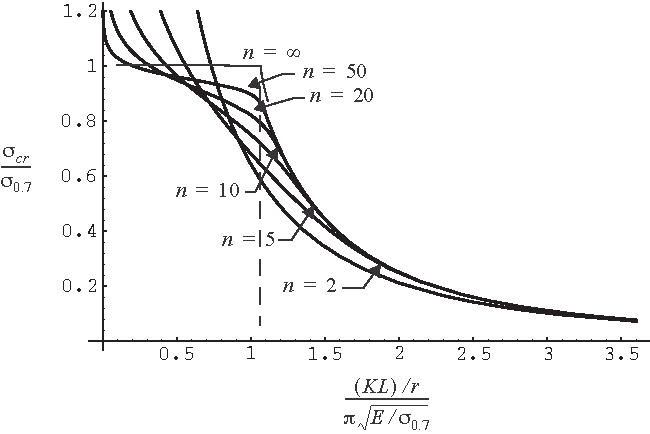
\includegraphics{Figure_11-21.pdf}}
\caption{Column curves for a Ramberg-Osgood material law with different shape factors.} \label{fig11.21}
\vspace*{-1.6pc}
\end{figure}

\section{Bending of thin plates}\label{sec11.6}

Recall that bars and beams are structural elements characterized by having two orthogonal dimensions, say the thickness and width, that are small compared to the third orthogonal dimension, the length. Thin plates, both flat and curved, are common structural elements in flight vehicle structures, and they are characterized by one dimension being small, say the thickness, with respect to the other two orthogonal dimensions, say the width and length. A thin, rectangular, flat plate shown in figure~\ref{fig11.22} is referenced to Cartesian axes $x$, $y$, and $z$, where the $x$-direction is parallel to the length, the $y$-direction is parallel to the width, and the $z$-axis is parallel to the thickness of the plate. We denote the length of the plate by $a$, the width by $b$, and the thickness by $t$, and $0 \leq x \leq a$, $0 \leq y \leq b$, and $-t/2 \leq z \leq t/2$. The plane with $z=0$ is the midsurface, or reference surface, of the plate.

\begin{figure}[!h]\vspace{-4pt}
\centerline{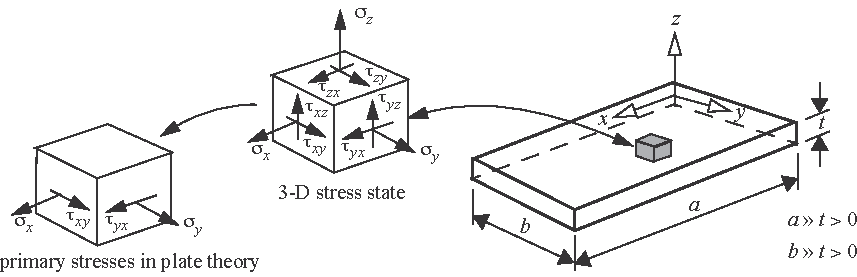
\includegraphics{Figure_11-22.pdf}}
\caption{Illustration of the nomenclature and primary stresses for a flat, rectangular plate.} \label{fig11.22}\vspace*{-4pt}
\end{figure}

A beam resists the transverse loads, or lateral loads, primarily by the longitudinal normal stress $\sigma_{{x}}$, and the so-called lateral stresses $\sigma_{{y}}$, $\sigma_{{z}}$, $\tau_{{yx}}$, and $\tau_{{yz}}$ are assumed to be negligible. Transverse loads, acting in\vadjust{\vspace*{8pt}\pagebreak} the $z$-direction applied to the plate are primarily resisted by the in-plane stress components $\sigma_{{x}}$, $\sigma_{{y}}$, and $\tau_{{xy}}$. Transverse shear stresses $\tau_{{xz}}$ and $\tau_{{yz}}$ are necessary for force equilibrium in the $z$-direction under transverse loads, but are smaller in magnitude with respect to the in-plane stresses. In plate theory, the transverse normal stress $\sigma_{{z}}$ is very small with respect to the in-plane normal stresses and, hence, is neglected. Bending of thin plates is discussed in many texts on plate theory; for example, see Ugural and Fenster (2003). Only some elements of the plate bending theory are discussed here. The assumptions of the linear theory for thin plates are as follows:
\begin{enumerate}
\item The deflection of the midsurface is small with respect to the thickness of the plate, and the slope of the deflected midsurface is much less than unity.
\item Straight lines normal to the midsurface in the undeformed plate remain straight and normal to the midsurface in the deformed plate, and do not change length.
\item The normal stress component $\sigma_{{z}}$ is negligible with respect to the in-plane normal stresses and is neglected in Hooke's law.
\end{enumerate}

Now consider the deformation, or strains, caused by the normal stresses. Hooke's law for the normal stresses and strains in a three-dimensional state of stress\vspace*{-3pt} is
\begin{align}\label{eq11.102}
\begin{aligned} \varepsilon_{x} &=\frac{1}{E}\left(\sigma_{x}-v \sigma_{y}-v \sigma_{z}\right) \\ \varepsilon_{y} &=\frac{1}{E}\left(-v \sigma_{x}+\sigma_{y}-v \sigma_{z}\right) \\ \varepsilon_{z} &=\frac{1}{E}\left(-v \sigma_{x}-v \sigma_{y}+\sigma_{z}\right) \end{aligned},
\end{align}
where $E$ is the modulus of elasticity and $v$ is Poisson's ratio. From assumption \textbf{3} the thickness normal stress $\sigma_{\textrm{z}}$ is assumed negligible and is set to zero in Hooke's law. From assumption \textbf{2} the thickness normal strain $\varepsilon_{z}=0$, because the line element normal to the midsurface does not change length. Since the normal stress $\sigma_{z}$ is also assumed to vanish, the third of eq.~(\ref{eq11.102}) leads to a contradiction. Hence, the third equation of Hooke's law is neglected. The material law for the in-plane normal strains and stresses for thin plates\vspace*{-3pt} is
\begin{align}\label{eq11.103}
\begin{aligned} \varepsilon_{x} &=\frac{1}{E}\left(\sigma_{x}-v \sigma_{y}\right) \\ \varepsilon_{y} &=\frac{1}{E}\left(-v \sigma_{x}+\sigma_{y}\right)\end{aligned}.
\end{align}

\vspace*{-1pc}

Consider two cases of pure bending of a plate or a beam subject to moment $M$. In the first case the cross section is compact with dimension $b$ nearly equal to thickness $t$, and in the second case dimension $b$ is much larger than thickness $t$. In the first case the structure is a beam, and in the second case it is a plate. In pure bending the neutral axis of the beam deforms into an arc of a circle with radius $\rho$, and the normal strain in the $x$-direction is $\varepsilon_{x}=z/\rho$. Note that we assumed that the $x$-axis coincided with the neutral axis in the undeformed beam. Hence, longitudinal line elements above the neutral axis, $z>0$, are stretched, and line elements below the neutral axis, $z<0$, are compressed. In the case of a beam, the normal stress in the $y$-direction, $\sigma_{y}$, is also very small and is neglected with respect to the longitudinal normal stress $\sigma_{x}$. That is, the beam resists the applied bending moment by the longitudinal normal stress $\sigma_{x}$. Since $\sigma_{y}=0$, we get from Hooke's law, eq.~(\ref{eq11.103}),\vspace*{-3pt} that
\begin{align}\label{eq11.104}
\begin{gathered} \sigma_{x}=E \varepsilon_{x} \\
\varepsilon_{y}=-v \varepsilon_{x}=-\frac{v}{\rho} z=-\frac{z}{\left(\frac{\rho}{v}\right)} \end{gathered}.
\end{align}
Hence, the longitudinal normal stress is the modulus of elasticity times the longitudinal normal strain, and the normal strain in the $y$-direction is just Poisson's ratio times the longitudinal normal strain. The form\vadjust{\vspace*{8pt}\pagebreak} of the last expression for $\varepsilon_{{y}}$ in eq.~(\ref{eq11.104}) shows that the line elements in the cross section parallel to the $y$-axis before deformation also bend into circular arcs. The line element parallel to the $y$-direction at $z=0$ in the undeformed beam has a radius of curvature of $\frac{\rho}{v}$ in the deformed beam. This transverse curvature is called \textit{anticlastic curvature}, and is illustrated in figure~\ref{fig11.23}.

\begin{figure}[!h]\vspace*{-4pt}
\centerline{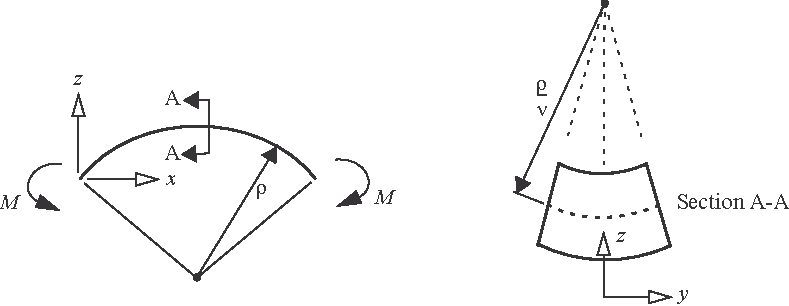
\includegraphics{Figure_11-23.pdf}}
\caption{Pure bending of a beam in the $x$-$z$ plane and the associated anticlastic curvature of its cross section.} \label{fig11.23}\vspace*{-4pt}
\end{figure}

Now consider pure bending of a plate under the same moment \textit{M}, where now the dimension $b$ is much larger than thickness $t$. In this case experiments show that the transverse line elements remain straight over the central section of the plate, so that the anticlastic curvature is suppressed. In this central section of the plate the transverse normal stress $\varepsilon_{{y}}$ is non-zero. However, the transverse normal stress must vanish at the free edges at $y=0$ and $y=b$, so that anticlastic curvature develops only in narrow zones near the free edges to adjust to vanishing of the normal stress $\sigma_{y}$ at the free edges. In the central portion of the plate, the associated normal strain is zero. The suppression of anticlastic curvature is characterized by the vanishing of the normal strain $\varepsilon_{{y}}$. Hence from Hooke's law, eq.~(\ref{eq11.103}), for $\varepsilon_{{y}} = 0$ we get
\begin{align}\label{eq11.105}
\sigma_{x}=\frac{E}{1-v^{2}} \varepsilon_{x} \quad \sigma_{y}=v \sigma_{x}.
\end{align}
Since the denominator in the expression for $\sigma_{{x}}$ is positive but less than unity, the plate is stiffer than the beam owing to the presence of the non-zero transverse normal stress $\sigma_{y}$ to help in resisting the applied moment. Compare eqs. (\ref{eq11.104}) and (\ref{eq11.105}) for the normal stress $\sigma_{{x}}$. The quantity $E /\left(1-v^{2}\right)$ is an effective modulus of the plate.

\begin{figure}[!h]
\centerline{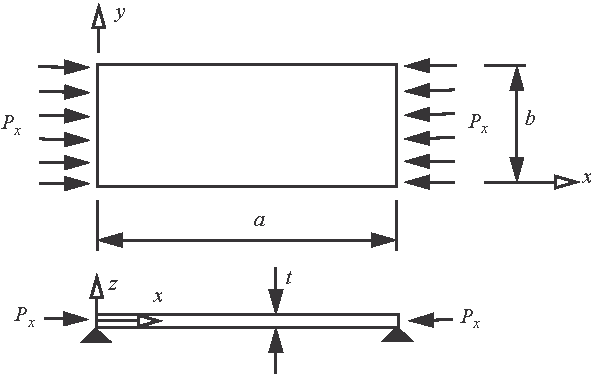
\includegraphics{Figure_11-24.pdf}}
\caption{Uniformly applied compressive forces applied to opposite longitudinal edges of a rectangular plate. } \label{fig11.24}
\end{figure}

\section{Compression buckling of thin rectangular plates}\label{sec11.7}

Consider the perfectly flat plate subject to a longitudinal compressive force of magnitude $P_{x}$ applied in a spatially uniform manner along edges $x=0$ and $x=a$, as shown in figure~\ref{fig11.24}. The equilibrium response of the plate in linear theory is that of pure compression in the \textit{x-y} plane with no out-of-plane deflection of the midsurface. That is, in the pre-buckling equilibrium state the plate remains flat. The normal stress $\sigma_{x}$ in the plate is spatially uniform, and we write it as $\sigma_{x}=-\sigma$, where $\sigma=P_{x}/(b t)$ is the applied compressive stress.

At a critical value of the compressive force $P_{xcr}$ the plate will buckle, or deflect out of the flat pre-buckling equilibrium state. To determine this critical force we have to consider a slightly deflected equilibrium configuration of the plate, similar to the analysis of the perfect column presented in article~\ref{sec11.1}. Refer to Brush and Almroth (1975) for the details of this adjacent equilibrium analysis for the critical force\vadjust{\vspace*{8pt}\pagebreak}.

Instead of a detailed adjacent equilibrium analysis of the plate, we can make a comparison to the critical force determined for the pinned-pinned column in figure~\ref{fig11.6}. The configuration of the plate comparable to the pinned-pinned column has simply supported, or hinged, edges at $x=0$ and $x=a$, and has free edges at $y=0$ and $y=b$. The compressively loaded plate for these boundary conditions is called a \textit{wide column.} The critical force for the pinned-pinned column is
\begin{align}\label{eq11.106}
P_{c r}=\pi^{2} \frac{E I}{L^{2}}.
\end{align}
For the plate, replace the modulus of elasticity $E$ in the column formula by $E /\left(1-v^{2}\right)$, since the plate is stiffer than the column. Also set $L=a$ for the plate. The formula for the second area moment of a rectangular cross section is $I=\left(b t^{3}\right)/12$. Hence, eq.~(\ref{eq11.106}) transforms to
\begin{align}\label{eq11.107}
P_{x c r}=\pi^{2}\left(\frac{E}{1-v^{2}}\right)\left(\frac{1}{a^{2}}\right)\left(\frac{b t^{3}}{12}\right)=\pi^{2}\left(\frac{E t^{3}}{12\left(1-v^{2}\right)}\right) \frac{b}{a^{2}}.
\end{align}
For the \textit{wide column} configuration of the plate, the critical load is written in the form
\begin{align}\label{eq11.108}
P_{x c r}=\frac{\pi^{2} D b}{a^{2}},
\end{align}
where the bending stiffness, or flexural rigidity, of the plate is defined as
\begin{align}\label{eq11.109}
D=\frac{E t^{3}}{12\left(1-v^{2}\right)}.
\end{align}
The critical compressive stress at buckling is simply $\sigma_{cr}=P_{xcr}/(bt)$. Divide eq.~(\ref{eq11.107}) by area \textit{bt} to get
\begin{align*}
\sigma_{c r}=\pi^{2}\left(\frac{E t^{3}}{12\left(1-v^{2}\right)}\right) \frac{b}{a^{2}} \frac{1}{b t}=\pi^{2} \frac{E}{12\left(1-v^{2}\right)}\left(\frac{t}{b}\right)^{2}\left(\frac{b}{a}\right)^{2}.
\end{align*}
By convention, this critical compressive stress is written in the form
\begin{align}
\boxed{\sigma_{c r}=k_{c} \pi^{2} \frac{E}{12\left(1-v^{2}\right)}\left(\frac{t}{b}\right)^{2}} \label{eq11.110}
\end{align}
where $k_{c}$ is a nondimensional buckling coefficient for compressive loading, which is a function of the plate aspect ratio $a/b$. For the unloaded edges free and the loaded edges simply supported, this buckling coefficient is
\begin{align}\label{eq11.111}
k_{c}=\frac{1}{(a/b)^{2}} \quad \text { wide column}.
\end{align}

\vspace*{-1pc}

For other support conditions on the edges $x=0$, $x=a$, $y=0$, and $y=b$, the critical compressive stress is also given by eq.~(\ref{eq11.110}) but the compressive bucking coefficient is a different function of the plate aspect ratio. The transition from column to plate as supports are added along the unloaded edges ($y=0$ and $y=b$) are depicted in figure~\ref{fig11.25} on page~\pageref{fig11.25}. The compressive buckling coefficient is plotted for various support conditions as shown in figure~\ref{fig11.26} on page~\pageref{fig11.26}. Note that some of the curves for the buckling coefficient exhibit cusps, or discontinuous slopes, at selected values of the plate aspect ratio. The cusps correspond to changes in the half wave length of the buckle pattern along the $x$-direction. In particular, for the plate with simple support on all four edges, case C in figure~\ref{fig11.26} on page~\pageref{fig11.26}, note that $k_{c}=4$ for integer aspect ratios.

\subsection{Simply supported rectangular plate}\label{sec11.7.1}

Consider a plate simply supported on all four edges and subject to uniform compressive on edges $x=0$ and $x=a$. In the pre-buckling equilibrium configuration the plate remains flat, $w_{0}(x, y)=0$, with a spatially uniform compressive stress equal to the applied compressive stress $\sigma$. From the method of adjacent equilibrium, the out-of-plane displacement of the plate at the onset of buckling is
\begin{align}\label{eq11.112}
w_{1}(x, y)=A_{1} \sin \left(\frac{m \pi x}{a}\right) \sin \left(\frac{n \pi y}{b}\right),
\end{align}
where $m$ and $n$ are positive integers and $A_{1}$ is an arbitrary amplitude. Integer $m$ corresponds to the number of half waves in the $x$-direction and integer $n$ corresponds to the number of half waves in the $y$-direction. Thus, specific values of integers $m$ and $n$ in eq.~(\ref{eq11.112}) characterize a buckling mode, and for each buckling mode there is a corresponding buckling stress. Equation (\ref{eq11.110}) is the formula for the compressive stress at buckling, with the compressive buckling coefficient given by
\begin{align}\label{eq11.113}
k_{c}=\left(\frac{m}{a/b}+n^{2} \frac{(a/b)}{m}\right)^{2} \quad m, n=1,2, \ldots.
\end{align}
The critical stress is the lowest buckling stress, which occurs for a certain choice of $m$ and $n$. Since $k_{c}$ is directly proportional to powers of integer $n$, the minimum value of $k_{c}$ occurs for $n=1$. Then minimum values of $k_{c}$ are related to $a/b$  and integer $m$ by
\begin{align}\label{eq11.114}
k_{c}=\left(\frac{m}{a/b}+\frac{(a/b)}{m}\right)^{2}.
\end{align}

\vspace*{-1pc}

Critical values of the compressive buckling coefficient as a function of a few aspect ratios are listed in table~\ref{tab11.4}.

These critical values of the compression buckling coefficient are plotted as case C in figure~\ref{fig11.26} on page~\pageref{fig11.26}. The buckling modes for three integer values of the aspect ratio are depicted in figure~\ref{fig11.27}. There is one half{\parfillskip=0pt\par}
\vspace*{8pt}
\pagebreak

\begin{figure}
%\thispagestyle{empty}
\vspace*{-7pt}
\centerline{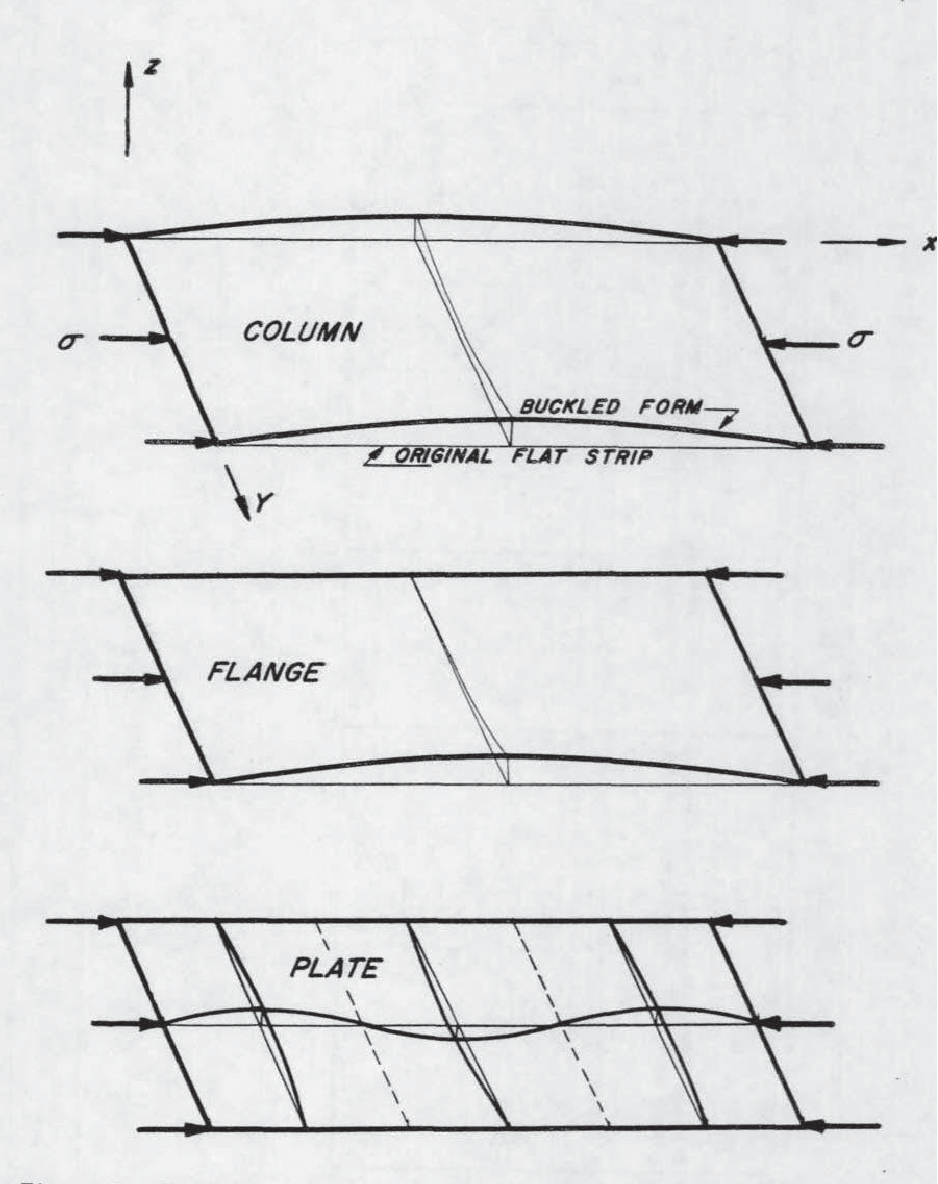
\includegraphics{Figure_11-25.pdf}}
\caption{Transition form column to plate as supports are added along unloaded edges. Note changes in buckle configurations (NACA TN 3781, figure 1).} \label{fig11.25}
\vspace*{7pt}
\end{figure}

\clearpage

\begin{figure}
\centerline{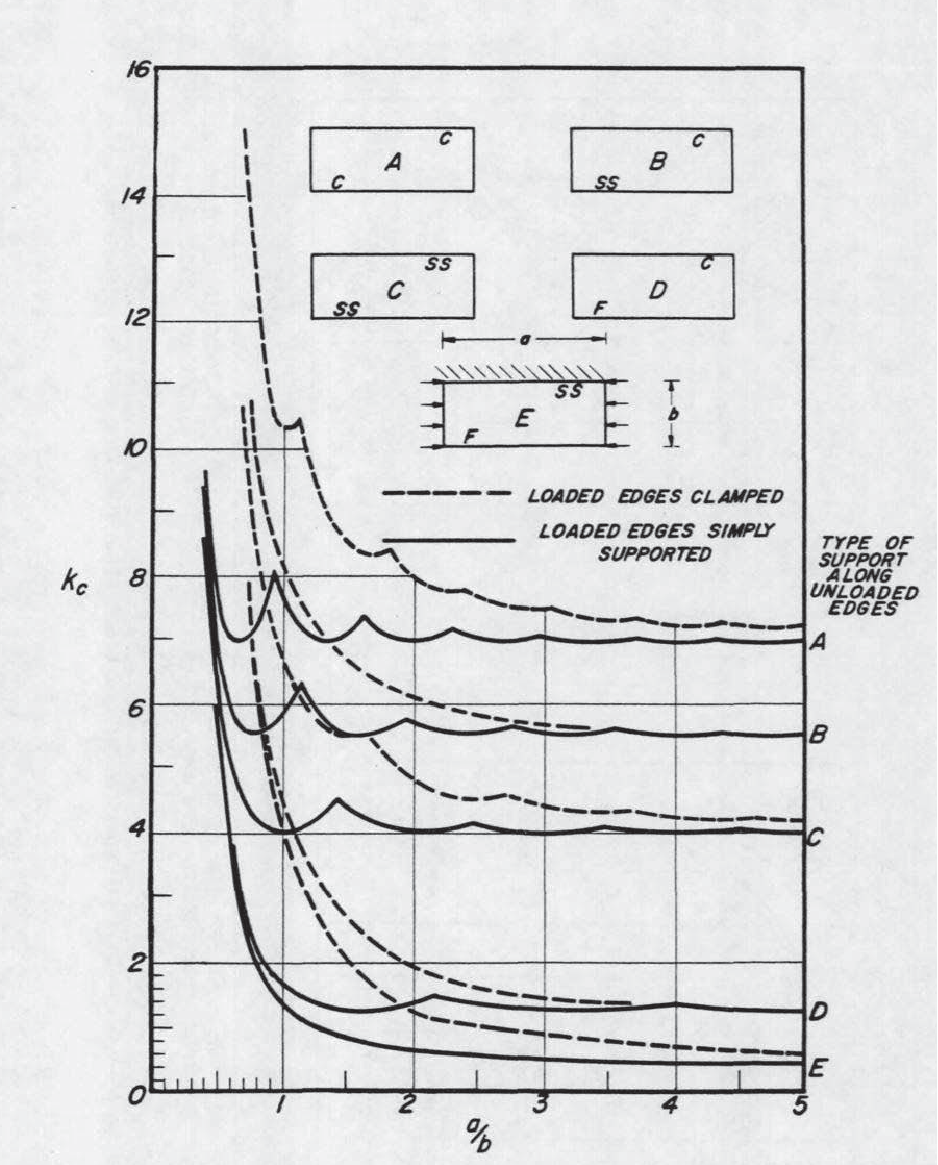
\includegraphics{Figure_11-26.pdf}}
\caption{Compression buckling coefficient for flat rectangular plates (NACA TN 3781, figure 14).} \label{fig11.26}
\end{figure}

\clearpage

\begin{table}[!t]
\processtable{Compression buckling coefficient for selected plate aspect ratios \label{tab11.4}}{
\tabcolsep=18pt\begin{tabular}{@{}lll@{}}
\toprule
\colhead{} & \colhead{Number of half waves} & \colhead{Critical compressive} \\
\colhead{Plate aspect ratio} & \colhead{in the $x$-direction} & \colhead{buckling coefficient} \\
\midrule
$0<a/b \leq \sqrt{2}$ & $m=1$ &  $k_{c r}=\left(\frac{1}{a/b}+\frac{a/b}{1}\right)^{2}$ \\[6pt]
$\sqrt{2} \leq a/b \leq \sqrt{6}$ & $m=2$ & $k_{c r}=\left(\frac{2}{a/b}+\frac{a/b}{2}\right)^{2}$ \\[6pt]
$\sqrt{6} \leq a/b \leq \sqrt{12}$ & $m=3$ & $k_{c r}=\left(\frac{3}{a/b}+\frac{a/b}{3}\right)^{2}$ \\
\botrule
\end{tabular}}{}
\vspace*{-0.7pc}
\end{table}

\noindent wave across the width ($n=1$) and the number of half waves across the length, $m$, increases with increasing aspect ratio. For integer values of the aspect ratio the critical value of the compressive buckling coefficient $k_{c r}=4$, and it follows that the critical compressive stress is
\begin{align}\label{eq11.115}
\sigma_{c r}=4 \pi^{2} \frac{E}{12\left(1-v^{2}\right)}\left(\frac{t}{b}\right)^{2} \quad \frac{a}{b}=m=1,2,3, \ldots \quad n=1.
\end{align}
From eq.~(\ref{eq11.112}) the length of a half wave in the $x$-direction is $a/m$, and the length of a half wave in the $y$-direction is the plate width $b$ for $n=1$. These half wave lengths are the same when $a/m=b$, or $a/b=m$. That is, the half wave lengths in the $x$- and $y$-directions are the same for integer values of the aspect ratio. Hence, for integer values of the plate aspect ratio the buckling mode consists of a sequence of \textit{square buckles}.

\begin{figure}[!h]
\centerline{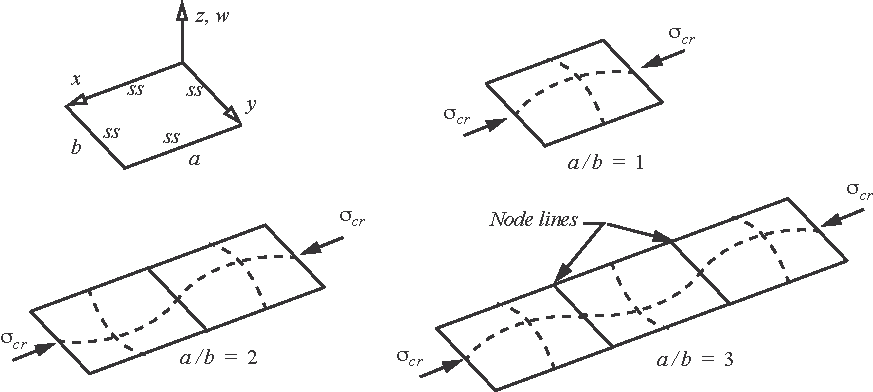
\includegraphics{Figure_11-27.pdf}}
\caption{Compression buckling modes for integer aspect ratios of a simply supported rectangular plate.} \label{fig11.27}
\end{figure}

\clearpage

\begin{example}[Critical load for simply supported rectangular plate in compression]\label{ex11.4}%
Let $a=20$\,in., $b=10$\,in., $t=0.10$\,in., $E=10 \times 10^{6}\,\textrm{lb}./\mathrm{in}.^{2}$, and $v=0.3$. From eq.~(\ref{eq11.110}) the critical compressive stress
\begin{align}
\sigma_{\mathrm{cr}}=k_{c}(903.81\,\textrm{lb}./\mathrm{in.}^{2}). \label{eq11.4.a}\tag{a}
\end{align}
From eq.~(\ref{eq11.114}) the compression buckling coefficient is
\begin{align}
k_{c}=\left(\frac{m}{2}+\frac{2}{m}\right)^{2}. \label{eq11.4.b}\tag{b}
\end{align}
For $m= 1, 2, 3, k_{c}=6.25,4.0,4.694$, respectively. For larger values of $m$, coefficient $k_{c}$ is larger. The minimum value of $k_{c}$ is 4 corresponding to $m=2$. Hence, the critical stress is
\begin{align}
\sigma_{\mathrm{cr}}=3,615.24\,\textrm{lb}./\mathrm{in.}^{2}. \label{eq11.4.c}\tag{c}
\end{align}
The critical compressive load $P_{\mathrm{cr}}=\sigma_{\mathrm{cr}} bt$. Hence,
\begin{align}
P_{\mathrm{cr}}=3{,}615\,\textrm{lb.}. \label{eq11.4.d}\tag{d}
\end{align}

\vspace*{-1pc}

The buckling mode for $(m, n)=(2,1)$ has one half sine wave in the transverse direction and two half waves in the longitudinal direction. The load $P_{\mathrm{cr}}=3{,}615\,\textrm{lb.}$ is the lowest load at which such a plate can lose its\break stability.
\end{example}

\begin{figure}[!b]
\centerline{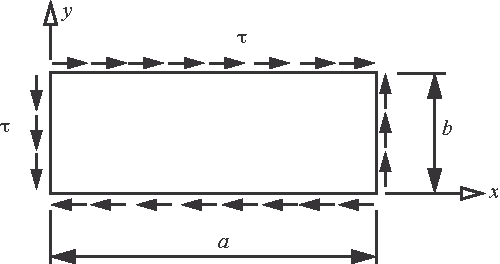
\includegraphics{Figure_11-28.pdf}}
\caption{Plate subject to in-plane shear loading.} \label{fig11.28}\vspace*{8pt}
\end{figure}


\section{Buckling of flat rectangular plates under shear loads}\label{sec11.8}

Consider a thin, rectangular plate with a thickness denoted by $t$, and the in-plane dimensions denoted by $a$ and $b$, where $0<t \ll b \leq a$. Note that $a$ denotes the long dimension of the plate and $b$ denotes the short dimension. It is subject to uniformly distributed shear stress $\tau$ as illustrated in figure~\ref{fig11.28}. From Mohr's circle for plane stress, the state of pure shear is equivalent to tensile and compressive normal stresses at forty-five degrees to the direction of pure shear. It is this compressive normal stress that leads to buckling of the thin plate subjected to shear.

The critical value of the shear stress per unit length, $\tau_{\mathrm{cr}}$, is given by the formula
\begin{align}\label{eq11.116}
\tau_{c r}=k_{s} \pi^{2} \frac{E}{12\left(1-v^{2}\right)}\left(\frac{t}{b}\right)^{2},
\end{align}
where $k_{s}$ is a nondimensional buckling coefficient for shear loading. This buckling coefficient is a function of the plate aspect ratio $a/b$ and the boundary conditions applied to the plate. Values of the shear buckling coefficient are given in figure~\ref{fig11.30} on page~\pageref{fig11.30}. The buckling mode labeled the symmetric mode in the figure pertains to a buckled form that is symmetric with respect to a diagonal across the plate at the node line slope. For a narrow range of aspect ratios the plate buckles in an antisymmetric mode. For an infinitely long strip, or $a/b \rightarrow \infty$, $k_{s}=5.35$ for simply supported, or hinged, edges at $y=0, b$, and $k_{s}=8.98$ for clamped edges.

A least squares fit of the shear buckling coefficient as a function of the plate aspect ratio is convenient in problem solving. For the simply supported plate, or the plate with hinged edges, the data listed in table~\ref{tab11.5} was read from the graph in figure~\ref{fig11.30}.

\begin{table}[!h]
\processtable{Shear buckling coefficient for selected plate aspect ratios \label{tab11.5}}{
\tabcolsep=45pt\begin{tabular}{@{}ll@{}}
\toprule
\colhead{\textit{a/b}} & \colhead{$\textit{k}_{\mbox{\scriptsize\bfseries\itshape s}}$} \\
\midrule
1 & 9.6\\
2 & 6.4\\
3 & 5.8\\
4 & 5.7\\
5 & 5.5\\
\botrule
\end{tabular}}{}
\end{table}

These data are fit to the functions 1 and $\frac{1}{a/b}$. The result of the least squares fit to these data is
\begin{align}\label{eq11.117}
k_{s}=4.22565+\frac{5.19931}{a/b} \quad 1 \leq a/b \leq 5.
\end{align}
The least squares fit and the input data are plotted in figure~\ref{fig11.29}.

\processfigure[!h]{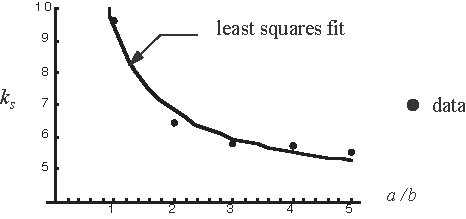
\includegraphics{Figure_11-29.pdf}}{\caption{Graph of eq.~(\ref{eq11.117}) compared to discrete data listed in table~\ref{tab11.5}.}\label{fig11.29}}

\clearpage

\begin{figure}
%\thispagestyle{empty}
\vspace*{-1.4pc}
\centerline{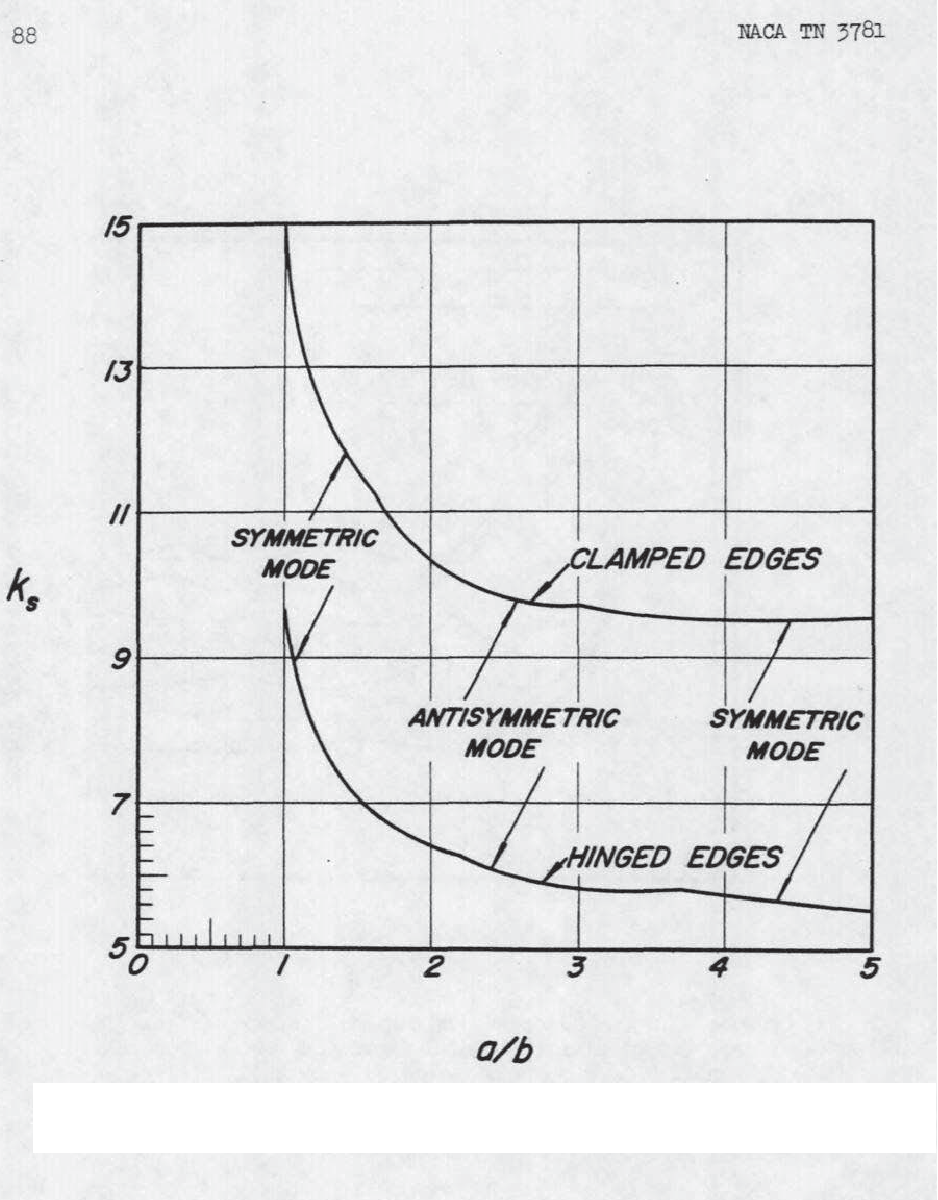
\includegraphics{Figure_11-30.pdf}}
\caption{Shear-buckling-stress coefficient of plates as a function of a/b for clamped and hinged edges (NACA TN 3781, figure 22).} \label{fig11.30}
\vspace*{1.4pc}
\end{figure}

\clearpage

\section{Buckling of flat rectangular plates under combined compression and shear}\label{sec11.9}

A plate subject to uniformly applied longitudinal compression and shear is shown in figure~\ref{fig11.31}. The critical combination of shear and compression stresses under different boundary conditions and different aspect ratios of the plate can be approximated to a sufficient accuracy by
\begin{figure}[!h]\vspace*{-4pt}
\centerline{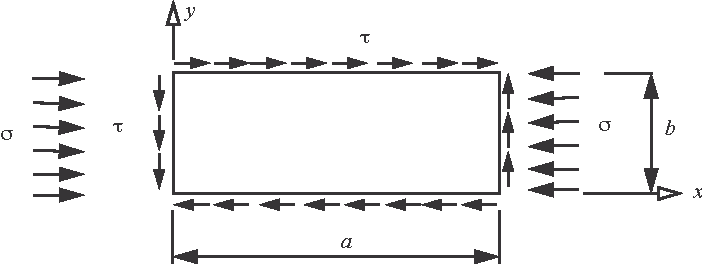
\includegraphics{Figure_11-31.pdf}}
\caption{Plate subject to longitudinal compression and in-plane shear loading.} \label{fig11.31}\vspace*{-8pt}
\end{figure}
\begin{align}\label{eq11.118}
\left(\frac{\tau}{\tau_{\textrm{cr}}}\right)^{2}+\left(\frac{\sigma}{\sigma_{\textrm{cr}}}\right)=1,
\end{align}
where $\tau_{\textrm{cr}}$ and $\sigma_{\textrm{cr}}$ are the critical values of the separately acting shear stress and the compression normal stress, respectively (NACA TN 3781, pp. 38, 39). Equation (\ref{eq11.118}) is plotted in figure~\ref{fig11.32}.



\begin{figure}[!h]
\centerline{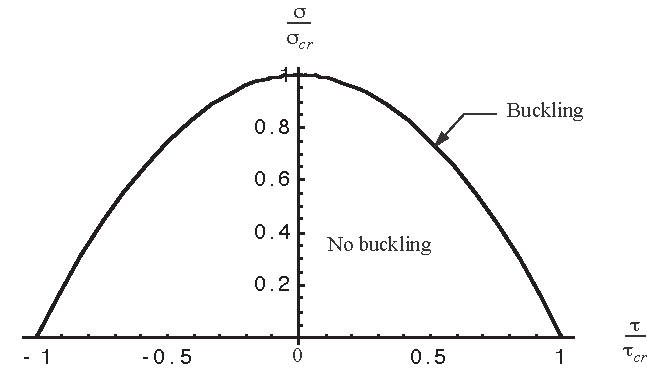
\includegraphics{Figure_11-32.pdf}}
\caption{Buckling interaction relationship for critical combinations of shear and compression.} \label{fig11.32}\vspace*{-8pt}
\end{figure}

\begin{example}[Wing rib spacing based on a buckling constraint]\label{ex11.5}The stringer stiffened box beam that is the main spar in a wing is shown in figure~\ref{fig11.33}. For a pull-up maneuver, the calculated transverse shear force $V_{y}=25{,}000\,\mathrm{lb}$. and the bending moment $M_{x}=-4.14 \times 10^{6}\,\textrm{lb}$--$\mathrm{in}$.\vadjust{\vspace*{8pt}\pagebreak} at the wing root. The thickness and width of the upper and lower cover skins are $t_{f}=0.5\,\textrm{in}$. and $b_{f}=24\,\mathrm{in}$., respectively. The thickness and height of the left and right webs are $t_{w}=0.30\,\textrm{in}$. and $b_{w}=13\,\textrm{in}$., respectively, and the flange area of the stringers $A_{f}=2.0 \text { in.}^{2}$. The material is isotropic with properties $E=10 \times 10^{6}\,\mathrm{lb}/\text{in.}^{2}$ and $v=0.3$. For $M_{x}<0$, the upper skin is in compression. Determine the rib spacing, denoted by $a$, such that the margin of safety for buckling of the upper skin is slightly positive.

\processfigure[!h]{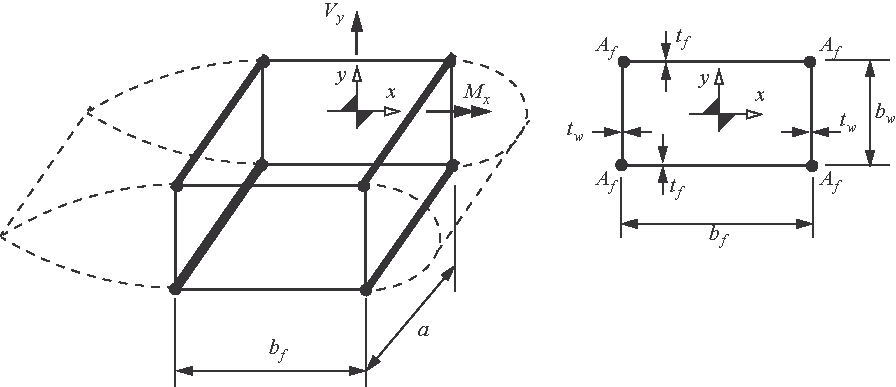
\includegraphics{Figure_11-33.pdf}}{\caption{Wing box beam of example~\ref{ex11.5}.}\label{fig11.33}}

\subsubsection{Solution.} The centroid and the shear center of the cross section coincide with the center of the box beam due to symmetry. The normal stress due to bending in the upper skin is calculated from the flexure formula; i.e.,
\begin{align}
\sigma_{z}=\frac{M_{x}\left(b_{w}/2\right)}{I_{x x}}, \label{eq11.5.a}\tag{a}
\end{align}
where the second area moment of the cross section about the $x$-axis is
\begin{align}
I_{x x}=b_{w}^{2} A_{f}+\frac{1}{2} b_{f} b_{w}^{2} t_{f}+\frac{1}{6} b_{w}^{3} t_{w}=1{,}461.85\,\mathrm{in}.^{4} \label{eq11.5.b}\tag{b}
\end{align}
Hence, the bending normal stress in the upper skin is
\begin{align}
\sigma_{z}=-18{,}408.2\,\textrm{lb}./\text {in.}^{2}. \label{eq11.5.c}\tag{c}
\end{align}

The shear stress in the upper skin is determined from the analysis of the shear flow distribution around the contour of the cross section, which is shown in figure~\ref{fig11.34}.

\processfigure[!h]{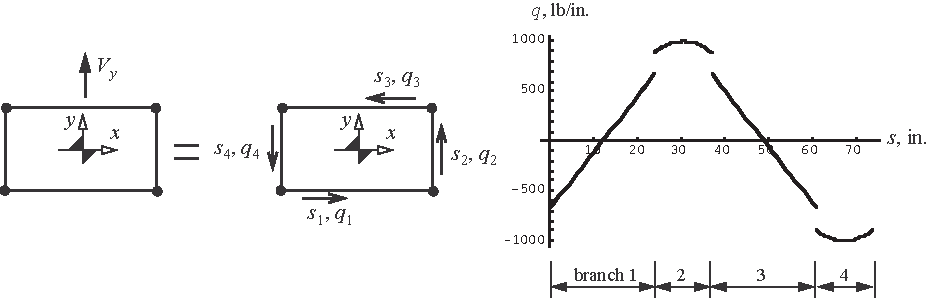
\includegraphics{Figure_11-34.pdf}}{\caption{Shear flow distribution for the box beam of example~\ref{ex11.5}.}\label{fig11.34}}

The shear flow in the upper skin is
\begin{align}
q_{3}=\frac{b_{w} t_{f}\left(b_{f}-2 s_{3}\right)}{4 I_{x x}} V_{y} \quad 0 \leq s_{3} \leq b_{f}. \label{eq11.5.d}\tag{d}
\end{align}
The shear stress $\tau_{3}=q_{3}/t_{f}$, and its evaluation is
\begin{align}
\tau_{3}=55.5803\left(24-2 s_{3}\right)\,\textrm{lb}./\text{in.}^{2} \quad 0 \leq s_{3} \leq 24\,\textrm{in}. \label{eq11.5.e}\tag{e}
\end{align}
Computing the maximum magnitude and the average value of this shear stress results in
\begin{align}
\left|\tau_{3}\right|_{\max}=1{,}333.93\,\textrm{lb}/\text{in.}^{2} \quad\left(\tau_{3}\right)_{\mathrm{ave}}=\frac{1}{b_{f}} \int_{0}^{b_{f}} \tau_{3} d s_{3}=0. \label{eq11.5.f}\tag{f}
\end{align}
The maximum magnitude of the shear stress in the upper skin is 7.25 percent of the magnitude of the bending normal stress. Moreover, the average value of the shear stress is zero in the upper skin. Hence, it is reasonable to neglect the effect of the shear stress on the buckling of the upper skin.

Assume the upper skin is a simply supported rectangular plate between the stringers and ribs. Actually, the stringer and ribs provide rotational constraint to the upper skin, but the assumption of no rotational constraint is conservative with respect to design. The critical compressive stress for simple support on all four edges of the upper skin underestimates its actual value. Equation (\ref{eq11.110}) for the top cover skin is
\begin{align}
\sigma_{\textrm{cr}}=k_{c} \pi^{2} \frac{E}{12\left(1-v^{2}\right)}\left(\frac{t_{f}}{b_{f}}\right)^{2}, \label{eq11.5.g}\tag{g}
\end{align}
and eq.~(\ref{eq11.114}) for the compression buckling coefficient is
\begin{align}
k_{c}=\left(\frac{m}{a/b_{f}}+\frac{a/b_{f}}{m}\right)^{2} \quad m \text { a positive integer to minimize } k_{c}. \label{eq11.5.aa}\tag{a}
\end{align}
The margin of safety is defined by
\begin{align}\label{eq11.119}
MS=\frac{\text { Excess strength }}{\text { Required strength }}=\frac{\sigma_{\mathrm{cr}}-\left|\sigma_{z}\right|}{\left|\sigma_{z}\right|}.
\end{align}
The margin of safety (\ref{eq11.119}) is positive for a feasible design, otherwise the design is infeasible. It should be a small positive value for a design of least weight. The computations for the margin of safety are listed in\break table~\ref{tab11.6}.

\begin{table}[!h]
\processtable{Margin of safety for selected rib spacings \label{tab11.6}}{
\tabcolsep=12pt\begin{tabular}{@{}llllll@{}}
\toprule
\colhead{a, in.} & \colhead{a/$\textbf{b}_{\textbf{f}}$} & \colhead{$\textbf{k}_{\textbf{c}}$} & \colhead{$\sigma_{\textrm{cr}}$, lb./in.$^{\textbf{2}}$} & \colhead{Margin of safety} & \colhead{Design} \\
\midrule
14 & 0.583  &  5.27905 &  20{,}708.6 &  \phantom{$-$}0.12497  &  feasible\\
15 &  0.625 &  4.95063 &  19{,}420.2 &  \phantom{$-$}0.05498 &  feasible\\
16 &  0.667 &  4.69444 &  18{,}415.3 &  \phantom{$-$}0.000387 &  feasible\\
17 &  0.708 &  4.49482 &  17{,}632.20 & $-$0.04215 &  infeasible\\
18 &  0.750 &  4.34028 &  17{,}026.0 & $-$0.07509 &  infeasible\\
19 &  0.792 &  4.2223 &  16{,}563.2 & $-$0.1002 &  infeasible\\
\botrule
\end{tabular}}{}
\vspace*{-1pc}
\end{table}

A rib spacing of 16 in. is a feasible design with a slightly positive margin of safety.
\end{example}

\begin{thebibliography}{}\label{sec11.10}
\bibitem{} Brush, D. O., and B. O. Almroth. \textit{\textbf{Buckling of Bars, Plates, and Shells}}. New York: McGraw-Hill, 1975, pp.\break 75--105.

\bibitem{} Budiansky, B., and J. W. Hutchinson. ``Dynamic Buckling of Imperfection-Sensitive Structures.'' In \textit{Proceedings of the Eleventh International Congress of Applied Mechanics} (Munich, Germany). 1964, pp. 639--643.

\bibitem{} Budiansky, B. ``Dynamic Buckling of Elastic Structures: Criteria and Estimates.'' In \textit{Proceedings of an International Conference at Northwestern University} (Evanston IL). New York and Oxford: Pergamon Press, 1966.

\bibitem{} Gerard, G., and H. Becker. \textit{\textbf{Handbook of Structural Stability: Part I, Buckling of Flat Plates}}. Technical Report NACA-TN 3781. Washington, DC: Office of Scientific and Technical Information, U.S. Department of Energy, 1957.

\bibitem{} Koiter, W. T. ``The Stability of Elastic Equilibrium.'' PhD diss., Teehische Hoog School, Delft, The Netherlands, 1945. (English translation published as Technical Report AFFDL-TR-70-25, Air Force Flight Dynamics Laboratory, Wright-Patterson Air Force Base, OH, February 1970.)

\bibitem{} National Advisory Committee for Aeronautics (NACA), Technical Note 3781 (NACA-TN-3781) July 1957. \url{https://ntrs.nasa.gov/api/citations/1930084505/downloads/19930084505.pdf}.

\bibitem{} Ramberg, W., and Osgood, W. \textit{Description of Stress-Strain Curves by Three Parameters}. Technical Report NACA-TN-902. Washington DC: NASA, 1943.

\bibitem{} Southwell, Richard V. ``On the Analysis of Experimental Observations in Problems of Elastic Stability.'' \textit{Proc. Roy. Soc. London} A, no. 135 (April 1932): 601--616.

\bibitem{} Timoshenko, S. P., and J. M. Gere. \textit{\textbf{Theory of Elastic Stability}}. New York: McGraw-Hill Book Company,1961, p.33.

\bibitem{} Ugural A. C., and S. K. Fenster. \textbf{Advanced Strength and Applied Elasticity}, 4th ed.,Upper Saddle River, NJ: Pearson Education, Inc., Publishing as Prentice Hall Professional Technical Reference, 2003, pp.\break 472--490.
\end{thebibliography}

\section{Practice exercises}\label{sec11.11}

\begin{exercise}
\begin{enumerate}[\textbf{2.}]
\item[\textbf{1.}] An ideal column of length \textit{L} is pinned at one end and fixed to a rigid bar of length $a$ at the other end. The second end of the rigid bar is pinned on rollers. Refer to figure~\ref{fig11.35} Find the critical load $P_{\mathrm{cr}}$ and discuss the extreme cases of $a \rightarrow 0$ and $a \rightarrow \infty$.
\vspace*{8pt}
\pagebreak

\processfigure[!h]{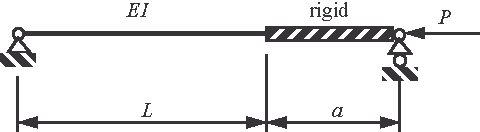
\includegraphics{Figure_11-35.pdf}}{\caption{Exercise 1.}\label{fig11.35}}

\item[\textbf{2.}] The column shown in figure~\ref{fig11.36} is pinned at the left end and supported by an extensional spring of stiffness $\alpha$ at the loaded right end.

\vspace*{-5pt}

\processfigure[!h]{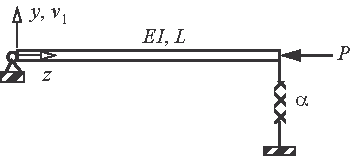
\includegraphics{Figure_11-36.pdf}}{\caption{Exercise 2.}\label{fig11.36}}

\begin{enumerate}[b)]
\item[{\hskip13pt}a)] Use the \textbf{adjacent equilibrium method} to show that the characteristic equation is
\begin{align*}
-k^{2} \sin k L\left[-k^{2}+\frac{\alpha L}{E I}\right]=0.
\end{align*}

\item[{\hskip13pt}b)] Plot the critical load $P_{\mathrm{cr}}$ as a function of $\alpha$, $0 \leq \alpha$. For what values of $\alpha$ will the column buckle in the Euler mode? (i.e., case~A in figure~\ref{fig11.6}).

\vspace*{-10pt}

\processfigure[!h]{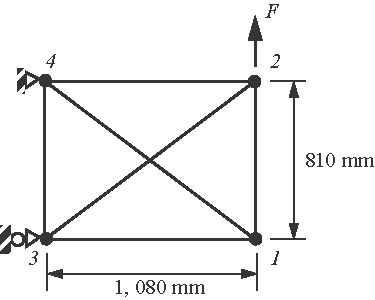
\includegraphics{Figure_11-37.pdf}}{\caption{Truss for exercise 3.}\label{fig11.37}}
\end{enumerate}
\vspace*{-12pt}


\item[\textbf{3.}] The statically indeterminate truss shown in figure~\ref{fig11.37} consists of six bars, labeled 1-2, 1-3, 1-4, 2-3, 2-4, and 3-4. It is subject to a vertical force \textit{F} at joint number~2. The cross-sectional area of each bar is 2{,}000\,mm$^{2}$, the second area moment of each bar is 160{,}000\,mm$^{4}$, and the modulus of elasticity of each bar is 75{,}000\,N/mm$^{2}$.



\begin{enumerate}[b)]
\item[{\hskip13pt}a)] Take bar force 1-4 as the redundant (i.e., $N_{1-4}=Q$). Using Castigliano's second theorem to determine the redundant \textit{Q} in terms of the external load \textit{F}.

\item[{\hskip13pt}b)] Determine the value of \textit{F} in kN to initiate buckling of the truss.

\item[{\hskip13pt}c)] If the yield strength of the material is 400 MPa in tension, determine the value of \textit{F} in kN to initiate yielding of the truss\vadjust{\vspace*{8pt}\pagebreak}.
\end{enumerate}

\item[\textbf{4.}] Bars 1-2, 2-3, and 2-4 of the truss shown figure~\ref{fig11.38} are unstressed at the ambient temperature. Only bar 1-2 is heated above the ambient temperature. Determine the increase in temperature, denoted by $\Delta T$, of bar 1-2 to cause buckling of the truss. The cross section of each bar is a thin-walled tube with radius $R=13\,\mathrm{mm}$ and wall thickness $t=1.5\,\mathrm{mm}$. Take length $L=762\,\mathrm{mm}$. All three bars are made of the same material with properties $E=75{,}000\,\mathrm{N}/\mathrm{mm}^{2}$ and $\alpha=23 \times 10^{-6} /{ }^{\circ}\mathrm{C}$.

\begin{figure}[!h]
\centerline{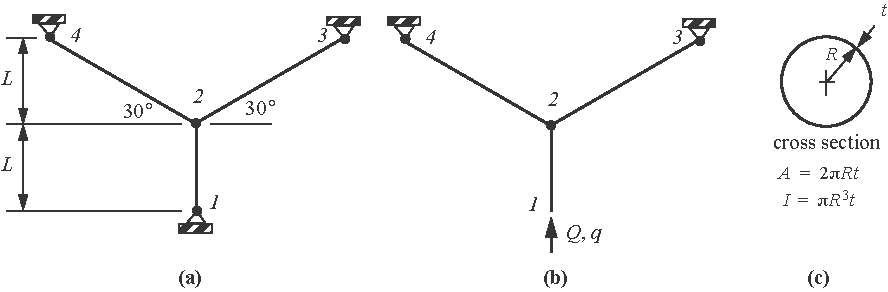
\includegraphics{Figure_11-38.pdf}}
\caption{Exercise 4. (a) three-bar truss, (b) base structure. (c) cross section of the bars.} \label{fig11.38}
\end{figure}

\item[\textbf{5.}] Consider the wing spar in example~\ref{ex11.5}. A counterclockwise torque $T=6 \times 10^{6}\,\textrm{lb.}$-$\mathrm{in}$. is specified to act at the root cross section in addition to the specified transverse shear force and bending moment. Determine the rib spacing, denoted by $a$, such that the margin of safety with respect to buckling of the upper skin is slightly positive. Report the value of $a$ to two significant figures and the associated margin of safety. The margin of safety is defined by the formula\vspace*{-6pt}
\begin{align*}
\textit{MS}=\frac{1-f_{b}}{f_{b}} \quad \text { where } \quad f_{b}=\left(\frac{\tau}{\tau_{\textrm{cr}}}\right)^{2}+\frac{\sigma}{\sigma_{\textrm{cr}}}.
\end{align*}
Use the average value of the shear stress over the width of the upper skin for the shear stress $\tau$ in the margin of safety formula. Remember that dimension $b$ is smaller than dimension $a$ in the formula for the critical value of the shear stress, and that $b$ is the width of the plate/skin on which the compressive normal stress acts in the formula for $\sigma_{\mathrm{cr}}$.
\end{enumerate}
\end{exercise}


\end{document}